\documentclass{llncs}

\usepackage{llncsdoc}
\usepackage{graphicx}
\usepackage{float}
\usepackage{algorithmicx}
\usepackage{algorithm}
\usepackage{algpseudocode}
\usepackage{amsmath,amssymb,stmaryrd}
\usepackage{soul}
\usepackage{color}
\usepackage{tikz}
%\usepackage{subfigure}
\usepackage{subfig}
\usepackage{hyperref}
\usepackage{times}

\newcommand{\LD}{\langle}
\newcommand{\RD}{\rangle}
\def\Rset{\mathbb{R}}
\def\Rsetgeq{\mathbb{R}_{\geq 0}}
\def\Rsetge{\mathbb{R}_{> 0}}

\newcommand{\aistis}[1]{\marginpar{\footnotesize \color{red} {\bf A:} \textsf{#1}}}
\newcommand{\taolue}[1]{\marginpar{\footnotesize \color{red} {\bf TL:} \textsf{#1}}}
\newcommand{\dave}[1]{\marginpar{\footnotesize \color{red} {\bf D:} \textsf{#1}}}
\newcommand{\comment}[1]{\marginpar{\footnotesize \color{red} \textsf{#1}}}

\newcommand{\prismcomment}[1]{\mbox{\em #1}}
\newcommand{\prismkeyword}[1]{\mathtt{#1}}
\newcommand{\prismident}[1]{\mathit{#1}}
\newcommand{\prismtab}{\hspace*{0.5cm}}

\begin{document}

\title{Verifying Team Formation Protocols in PRISM\thanks{This work is supported by
the ERC Advanced Grant VERIWARE.}}
\author{Taolue Chen \and Marta Kwiatkowska \and David Parker \and Aistis Simaitis}
\institute{
  Computing Laboratory, University of Oxford\\
  Wolfson Building, Parks Road, Oxford, OX1 3QD, UK
  %Oxford University Computing Laboratory, Parks Road, Oxford, OX1 3QD, UK
}
\email{}

\maketitle
\vspace{-10pt}
\begin{abstract}
Multi-agent systems are an increasingly important software paradigm and in many of
its applications agents cooperate to achieve a particular goal.
This requires the design of efficient collaboration protocols,
a typical example of which is \emph{team formation}.
In this paper, we illustrate how probabilistic model checking,
a technique for formal verification of probabilistic systems,
can be applied to the analysis, design and verification of such protocols.
We start by analysing the performance of an existing team formation protocol
modelled as a discrete-time Markov chain.
Then, using a Markov decision process model,
we construct optimal algorithms for team formation,
with respect to both individual agents and the combined set of all agents.
Finally, we use stochastic two-player games to analyse the competitive coalitional setting,
in which agents are split into cooperative and hostile classes.
We present experimental results from these models
using the probabilistic model checking tool PRISM,
which we have extended with support for stochastic games.
\end{abstract}
\vspace{-25pt}
\section{Introduction}
\vspace{-5pt}
%\taolue{NB. I introduced the following abbreviations: Sec. for section, Alg. for Algorithm, and so on. Also, Eqn. for equation, and I use eqref
%to refer to an equation.}%
Multi-agent systems have become an important software paradigm. One of the
key ideas behind this approach is that several different agents can cooperate to achieve certain goals.
This requires the design of efficient collaboration protocols, of which \emph{team formation} is a typical example. In this paper, we focus on a distributed team formation protocol introduced in \cite{gaston2005agent}. There, the authors used it to analyse team performance in dynamic networks.
The protocol %was studied further in \cite{glinton2008agent}, and
has also been applied to coalition formation for data fusion in sensor networks \cite{glinton2008agent}. In both cases it has been used as a basis for designing other algorithms, which makes it a compelling target for formal analysis.

The basic setting for the protocol of \cite{gaston2005agent} consists of an \emph{agent organisation}, i.e., a network of interconnected agents which have certain resources. These agents attempt to form teams in order to accomplish tasks which are generated periodically and globally advertised to the agent organisation. The topology of the network restricts the set of possible agent teams -- for an agent to be on a team, the agent must have a connection with at least one other agent in that team. Tasks are generic in that they only require a team of agents with the necessary resources to accomplish the specific task. As in \cite{gaston2005agent}, we do not consider the solution process, but only the team formation.

\emph{Formal verification} is an approach to check the correctness of a system
using rigorous, mathematical reasoning.
Fully automated verification techniques such as \emph{model checking}
have proved to be widely applicable,
including to multi-agent systems \cite{lomuscio2006mcmas}.
In this paper, the systems that we study exhibit \emph{probabilistic} behaviour,
for example because the likelihood of certain tasks being generated follows a known distribution,
or because the algorithms employed by individual agents are randomised.
Thus, we use \emph{probabilistic model checking}, an automated technique for
the formal verification of \emph{stochastic} systems.

%It can, for example,
%calculate the likelihood of the occurrence of certain events
%during the execution of a system, and can be useful to establish performance
%measures. It is based on the construction and analysis of a
%mathematical model of the system, usually from a specification
%in some high-level description language. This model
%generally comprises a set of states, representing all the possible
%configurations of the system, the transitions that can
%occur between these states, and information about when and
%with what probability each transition will occur, and a probabilistic model checker applies algorithmic techniques to analyze the state space and calculate performance measures.

Probabilistic model checking is based
on the construction of a probabilistic model from a precise,
high-level description of a system's behaviour.
The model is then analysed against one or more formally specified \emph{quantitative} properties,
usually expressed in temporal logic.
These properties capture not just the \emph{correctness} of the system,
but a wide range of measures such as \emph{reliability} or \emph{performance}.
We can compute, for example, ``the probability that the algorithm successfully terminates within $k$ rounds''.
By augmenting the model with \emph{rewards}, a further range of properties can be analysed.

In addition to offering convenient high-level formalisms for representing models and their properties,
the strength of probabilistic model checking is that offers \emph{exact}, \emph{exhaustive} analysis techniques.
Rather than, for example, discrete-event simulation
(as it is done for team formation protocols in \cite{gaston2005agent}),
probabilistic model checking is based on an exhaustive exploration and numerical solution of the model,
allowing best- and worst-case behaviour to be identified.
This is particularly valuable for distributed protocols (like the ones in this paper),
whose behaviour is notoriously difficult to understand precisely. %inherently,
%\dave{add back? "formally analysing a small system can be of great help to obtain a better understanding of large ones."}
Furthermore, efficient techniques and tools exist for this purpose.

In this paper, we use the PRISM probabilistic model checker \cite{KNP11} to analyse various agent organisations for the team formation protocol of \cite{gaston2005agent}.
We use several different types of probabilistic models
and express quantitative performance properties of them in temporal logic.
Firstly, we model the original version of the protocol using discrete-time Markov chains (DTMCs), where the behaviour of each agent is described entirely in a probabilistic (deterministic) way. Then, we extend the original algorithm  by allowing agents to make decisions nondeterministically, instead of randomly, when forming teams; such systems are naturally modelled by Markov decision processes (MDPs). By analysing the MDP, we obtain the best- and worst-case performance of agent organisations.
MDPs, however, can only model fully collaborative behaviour, whereas in many scenarios it is crucial to address hostile behaviour of some agents in the organisation. To cater for this we use stochastic two-player games (STPGs) as a model for the system containing two groups of agents -- collaborative and hostile -- which try to, respectively, maximise or minimise the performance of the organisation. Orthogonal to these, we consider two different settings, namely \emph{offline} and \emph{online}, depending on whether the tasks are generated respectively \emph{before} and \emph{after} teams have formed (see Alg.~\ref{alg:main_process}).


Our experiments illustrate several aspects of agent organisation analysis. As a typical case, we choose four network topologies, each consisting of five agents, i.e., fully connected, ring, star, and a network having one isolated agent. For each one, we compute the expected performance of the organisation and find organisation-optimal resource allocation among agents. Then we show using MDP model checking what is the best performance that can be achieved by this organisation. Then we take the model to the STPG setting to obtain the optimal coalitions of different sizes and evaluate their performance. For all of these cases, we consider the offline and online dichotomy.

%\comment{resource v.s. skill?}
%
%\comment{add several advantages of our approach - base on results. }

%Comparing to the traditional simulation-based analysis, we think one of the greatest advantages of our work lies in that we can actually synthesize the best strategies for agents to achieve the optimal performances. Note that in \cite{gaston2005agent},  Our work on extensions of the \textsc{TeamJoin} algorithm and the analysis of the associated MDP and STPG models can be seen as a partial solution to this problem. Moreover, our experience indicates that by simply adapting the PRISM code, one could analyse the behaviour of different agent organisations very easily, which can be considered as another advantage.

%\paragraph{Contributions.}
In summary, the main contributions of this paper are as follows:
\begin{enumerate}
  \renewcommand{\labelenumi}{(\arabic{enumi})}
  \item We perform a comprehensive and \emph{formal} analysis of the performance of the team formation protocol proposed in \cite{gaston2005agent}.

  \item  We \emph{extend} the original algorithm of \cite{gaston2005agent}, allowing agents to make decisions nondeterministically when forming teams. Then, by modelling and analysing as an MDP, we \emph{synthesise} the best strategies for agents to achieve optimal performance, partially solving an open problem posed in \cite{gaston2005agent}.\footnote{We quote: ``the problem of developing or learning effective team initialising and team joining policies is also important, and is included in our on-going and future work".}

  \item  We address the competitive coalitional setting, in which agents are split into cooperative and hostile classes, using \emph{stochastic games} to synthesise optimal agent coalitions. To the best of our knowledge, this is the first work to perform a \emph{fully-automated} analysis of this kind.

  \item We extend the  PRISM model checker with support for modelling and automated analysis of STPGs;
  this is of independent interest.
\end{enumerate}
%
We note that it would be difficult to achieve (2) and (3) using simulation-based approaches;
this demonstrates the strength of formal verification.

\paragraph{Related work.} Cooperative behaviour, which is one of the greatest advantages of agent-based computing, has been studied from many different angles over the years.
Coalitional games have traditionally been analysed from a game-theoretic perspective \cite{osborne1994course}, but in recent years have attracted a lot of attention from researchers in artificial intelligence, especially in cooperative task completion \cite{shehory1998methods}.
Several approaches for team formation and collaborative task solving have been considered including team formation under uncertainty using simple heuristic rules \cite{kraus2003coalition}, reinforcement learning techniques \cite{abdallah2004organization} and methods using distributed graph algorithms \cite{manisterski2006forming}.
To reason formally about cooperative games, several logics (e.g., Alternating Time Logic \cite{AlurHK02}, Coalitional Game Logic \cite{agotnes2009reasoning}, Strategy Logic \cite{chatterjee2007strategy}) and other formalisms (e.g., Cooperative Boolean Games \cite{dunne2008cooperative}) have been introduced and used to analyse coalitional behaviour \cite{bonzon2007efficient}.
Model checking has been used to analyse (non-probabilistic) knowledge-based properties of multi-agent systems,
using the tool MCMAS \cite{lomuscio2006mcmas}.
%e.g., for classic problems like dining cryptographers \cite{lomuscio2006mcmas}.
Probabilistic model checking was employed to
analyse probabilistic agents in negotiation protocols \cite{BFW06b}
(but only for fixed strategies modelled as DTMCs)
and to Byzantine agreement protocols \cite{KN02}
(but not in a game- or agent-based setting).
%some protocols related to multi-agent system, for instance, clock synchronisation in wireless sensor networks using %Uppaal \cite{heidarian2009analysis}, Gossip \cite{KNP08d} and Byzantine agreement protocols \cite{KN02} using PRISM %\cite{KNP11}.
%\paragraph{Structure.}
\vspace{-10pt}
\section{Preliminaries}
\vspace{-5pt}
%In this paper, we shall us discrete-time
%Markov chains (DTMCs), Markov decision processes (MDPs), and Stochastic Two-Player Games (STPGs) as the modeling %formalism. %where time is modelled as
%%discrete steps and the probability of making each transition
%%is given by a discrete probability distribution.
%Below we give a short introduction on these models.

%----------------------------------------------------------------------------------------------------------------

\subsection{Probabilistic Models}

We begin with a brief introduction to the three different types of probabilistic models
that we will use in this paper.

%\vskip5pt
\emph{Discrete-time Markov chains} (DTMCs) are the simplest of these models.
A DTMC $(S,\mathbf{P})$ is defined by a set of states $S$ and a probability transition matrix
$\mathbf{P} : S\times S \rightarrow [0, 1]$, where $\sum_{s'\in S} \mathbf{P}(s, s') = 1$ for all $s \in  S$.
This gives the probability $\mathbf{P}(s, s')$ that a transition will take place from state $s$ to state $s'$.

%\vskip5pt
\emph{Markov decision processes} (MDPs) extend DTMCs by incorporating \emph{nondeterministic choice}
in addition to probabilistic behaviour.
An MDP $(S,Act,Steps)$ comprises a set of actions $Act$
and a (partial) probabilistic transition function $Steps:S\times Act\rightarrow Dist(S)$,
which maps state-action pairs to probability distributions over the state space $S$.
In each state $s\in S$, one or more distinct actions can be taken and, assuming that action $a\in Act$ is chosen,
the distribution $Steps(s,a)$ gives the probability of making a transition to each state.

%Markov Decision Processes (MDP) allow accurate modelling of systems which exhibit
%both probabilistic and nondeterministic behaviour. Formally, a Markov decision process (MDP) is a tuple $(S, s_0, Act, %Steps)$ where $S$ is a finite set of states,
%$s_0$ is the initial state, $Act$ is a set of actions
%and $Steps\subseteq S \times Act \times Dist(S)$ is a probabilistic transition relation.
%An MDP transition $s\stackrel{a,\mu}s'$ is made from a state $s\in S$ first by nondeterministically
%selecting an action-distribution pair $(a, \mu)$ such that $(s, a, \mu) \in
%steps$, and second by making a probabilistic choice of the target state $s'$ according to the distribution
%$\mu$, such that $\mu(s') > 0$. A path represents a particular

%An \emph{adversary} represents a particular resolution
%of nondeterminism only. Formally, an adversary of a MDP is a function $A$
%mapping every finite path $\pi$ to a pair $(a, \mu)$ such that $(last(\pi), a, \mu)\in Steps$.
%The evolution of the MDP according to a particular adversary $A$ is a
%measurable set of infinite paths associated with $A$, which can classically be
%provided with a probability measure.

%\vskip5pt
\emph{Stochastic two-player games} (STPGs) generalise MDPs by allowing the nondeterministic choices
in the model to be resolved by two distinct players.
An STPG is a tuple $(S,(S_1,S_2),Act,Steps)$
where the set of states $S$ is partitioned into two disjoint subsets $S_1$ and $S_2$.
As for MDPs, $Steps:S\times Act\rightarrow Dist(S)$ is a function mapping
state-action pairs to distributions over states.
This is a \emph{turn-based} game. In each state $s$ of the game,
either player 1 or player 2 selects an action $a\in Act$,
depending on whether $s$ is in set $S_1$ or $S_2$.
%----------------------------------------------------------------------------------------------------------------
\vspace{-10pt}
\subsection{Probabilistic Model Checking \& PRISM}

Probabilistic model checking involves the construction and analysis of a probabilistic model.
Typically, a high-level description language is used to model a system
(here, we use the PRISM \cite{KNP11} modelling language).
Then, one or more quantitative properties are formally specified and analysed on the model.
Usually, \emph{probabilistic temporal logics} are used to formalise properties.
In this paper, we use PRISM's temporal logic-based query language,
which is essentially the logic PCTL \cite{HJ94},
extended to include reward-based properties \cite{KNP07a,FKNP11}.
This be used to express properties of both DTMCs and MDPs;
We also generalise the logic to capture properties of stochastic games.

PCTL extends the well known temporal logic CTL  with a probabilistic ($\tt P$) operator.
Informally, this places bounds on the probability of the occurrence of certain events in the model.
We will illustrate the use of PRISM temporal logic queries, using some simple examples,
referring the reader to \cite{HJ94,KNP07a} for precise details of the syntax and semantics.
For a DTMC, typical queries would be:
\vspace{-5pt}
\begin{itemize}
\item ${\tt P}_{<0.01}[\,\Diamond\,\mathit{fail}\,]$ -
``the probability of a failure occurring is less than 0.01''
\item ${\tt P}_{\geq 0.95}[\,\Diamond\,\mathit{end}\,]$ -
``the probability of the protocol terminating is at least 0.95''.
%\item ${\tt P}_{\geq 0.95}[\,\Diamond^{\leq 60}\,\mathit{end}\,]$ -
%``the probability of the protocol completing with 60 time units is at least 0.95''.
\end{itemize}
\vspace{-5pt}
For simplicity, we restrict our attention to \emph{reachability} queries
(in the examples above, $\mathit{fail}$ is a \emph{label}, denoting a particular subset of the DTMC's states $S$
and $\Diamond\,\mathit{fail}$ refers to the event in which a state from this set is reached).
%
In practice, we often use a \emph{quantitative} variant of the ${\tt P}$ operator,
denoted ${\tt P}_{=?}$, which returns the actual probability of an event's occurrence, e.g.:
\vspace{-5pt}
\begin{itemize}
\item ${\tt P}_{=?}[\,\Diamond\,\mathit{fail}\,]$ -
``what is the probability of a failure occurring?''
\end{itemize}
\vspace{-5pt}
Whereas in a DTMC it is relatively straightforward to define the probability
of an event such as $\Diamond\,\mathit{fail}$,
% or $\Diamond^{\leq 60}\,\mathit{end}$ in the examples above),
for MDPs we must also take account of the nondeterminism in the model.
The standard approach is to use the notion of
\emph{strategies} (also referred to as \emph{policies}, \emph{schedulers}, etc.).
A strategy resolves nondeterminism in an MDP (i.e. chooses an action in a state),
based on its execution history. % so far.
For a specific strategy, we \emph{can} define the probability of an event.
Thus, probabilistic model checking focuses on best- or worst-case analysis,
quantifying over all possible strategies.
We still employ quantitative properties,
which now ask for \emph{minimum} or \emph{maximum} probabilities:
\vspace{-5pt}
\begin{itemize}
\item ${\tt P}_{\max=?}[\,\Diamond\,\mathit{fail}\,]$ -
``what is the maximum probability of a failure occurring?''
\end{itemize}
\vspace{-5pt}
For a stochastic game, the same approach generalises naturally,
but we require strategies for both players.
Usually, we assume that the two players have opposing objectives,
for example player 1 aims to minimise the probability of $\Diamond\,\mathit{fail}$
and player 2 tries to maximise it.
Extending the notation from above, we write:
\vspace{-5pt}
\begin{itemize}
\item ${\tt P}_{\min,\max=?}[\,\Diamond\,\mathit{fail}\,]$ -
``what is the minimum probability of failure that player 1 can guarantee,
assuming that player 2 tries to maximise it?''
\end{itemize}
\vspace{-5pt}
%
For this simple class of (zero-sum) properties,
these values are well defined \cite{Con92}.

Finally, we also use properties based on \emph{rewards},
which capture a variety of additional quantitative measures.
For consistency across all three types of models,
we assume a simple state-based scheme,
i.e., a \emph{reward function} $\rho:S\rightarrow\Rsetgeq$.
We consider the \emph{expected total reward} accumulated until some target set of states is reached.
Consider a DTMC with reward function $\mathit{time}$
and a label $\mathit{end}$ denoting a set of target states.
We write, for example:
\vspace{-5pt}
\begin{itemize}
\item ${\tt R}^{\mathit{time}}_{=?}[\,\Diamond\,\mathit{end}\,]$ -
``what is the expected time for the algorithm to complete?''
\end{itemize}
\vspace{-5pt}
In exactly the same style as above, these queries generalise to MDPs and STPGs: %, e.g.:
\vspace{-5pt}
\begin{itemize}\addtolength{\itemsep}{2pt}
\item ${\tt R}^{\mathit{time}}_{\max=?}[\,\Diamond\,\mathit{end}\,]$ -
``what is the maximum expected algorithm completion time?''
\item ${\tt R}^{\mathit{time}}_{\min,\max=?}[\,\Diamond\,\mathit{end}\,]$ -
``what is the minimum expected time for algorithm completion
that player 1 can guarantee, assuming player 2 tries to maximise it?''
\end{itemize}
\vspace{-5pt}
\emph{PRISM} \cite{KNP11} is a probabilistic model checker.
It supports several different types of models, including DTMCs and MDPs
(it also supports continuous-time Markov chains and probabilistic timed automata).
On these models, a wide range of temporal logic-based properties can be checked,
including all of those illustrated above.
For the work presented here, we have built a prototype extension of PRISM
that adds support for STPGs.
Models to be analysed by PRISM are described in a
high-level modelling language based on guarded command notation;
we discuss this further in Section~\ref{sect:prismmodels}.
\vspace{-10pt}
\section{Definitions and Algorithms}
\vspace{-10pt}
The purpose of this section is to provide definitions of terminology
used throughout this paper and then present the algorithms which will be analysed.
\vspace{-10pt}
\subsection{Definitions}
\vspace{-5pt}
We introduce definitions of \emph{agent organisations}, \emph{tasks}, \emph{teams}, and formulae for computing \emph{rewards} to measure the performance of both individual agents and agent teams.
\begin{definition}[Agent Organisation]
An \emph{agent organisation} is a tuple $O=\langle A, N, R, R_A  \rangle$ where:
\vspace{-5pt}
\noindent
\begin{itemize}
\item $A= \{ a_1,a_2,...,a_n \} $ is a set of agents,
\item $N=\{\{a_i,a_j \}\ :$ ``$a_i$ and $a_j$ are neighbours'' $\}$ is a neighbourhood relation,
\item $R=\{r_1,r_2,\dots,r_k\}$ is a set of resource types, and
\item $R_A=\{R_{a_1}, R_{a_2}, \dots, R_{a_n}\}$ is a set of agent resources where $r_j \in R_{a_i} $ $\iff$ ``agent $a_i$ has a resource $r_j$''.
\end{itemize}
\vspace{-5pt}
\end{definition}

\begin{definition}[Task]
A \emph{task} $T_i=\{r_i\ :\ $``$r_i$ is required by the task $i$''$\}$ is a set of resources that are required to accomplish $T_i$. By $T=\{T_1, T_2,\dots, T_t\}$ we denote a collection of tasks.
\end{definition}

\begin{definition}[Team]
A \emph{team} of agents is denoted by $M_i=\{a_j\ :\ $``$a_j$ is a member of team $i$''$\}$, and the set of all teams is $M=\{M_1, M_2,\dots , M_m\}$. By $\bar{M} = \bigcup_{1\leq i\leq m} M_i$, we denote the set of all agents that are committed to some team. For $1\leq i\leq m$, $R_{M_i}=\bigcup_{a \in M_i}R_{a}$ is the set of resources the team $M_i$ has. The team $M_i$ is said to be able to accomplish the task $T_j$ iff $T_j \subseteq R_{M_i}$.
\end{definition}

\begin{definition}[Rewards]
For agent $a$, we define two types of \emph{reward}:
\vspace{-5pt}
\begin{itemize}
    \item Type $W_1$, which rewards the \emph{agent} with 1 point if it is in the team which was able to complete its task after team formation is over; and 0 otherwise. Formally,
\vspace{-5pt}
    \begin{equation} \label{eq:w1agent}
W_1(a) = \left\{
  \begin{array}{l l}
    1 & \quad \text{if $\exists M_i . a \in M_i \wedge T_i \subseteq R_{M_i}$,}\\
    0 & \quad \text{otherwise,}\\
  \end{array} \right.
\end{equation}
\vspace{-15pt}
    \item Type $W_2$, which rewards 1 point to the \emph{team} which was able to complete its task, and 0 otherwise. The reward is shared equally between team members.
\vspace{-5pt}
\begin{equation}
W_2(a) = \left\{
  \begin{array}{l l}
    \frac{1}{|M_i|} & \quad \text{if $\exists M_i . a \in M_i \wedge T_i \subseteq R_{M_i}$,}\\
    0 & \quad \text{otherwise.}\\
  \end{array} \right.
\label{eq:w2agent}
\end{equation}
\vspace{-5pt}
\end{itemize}
\vspace{-15pt}

For a set of agents $A$, the rewards are defined accordingly as the total reward achieved by its members, i.e.,
\vspace{-5pt}
\begin{equation} \label{eq:w1organisation}
 W_1(A) = \sum_{a \in A} W_1(a) \qquad
%
%\end{equation}
%\begin{equation}
 W_2(A) = \sum_{a \in A} W_2(a).
%\label{eq:w2organisation}
\end{equation}
\vspace{-20pt}
\end{definition}

The underlying idea of these two types of rewards is that $W_2$ provides
incentives for agents to form smaller teams which can accomplish tasks, whereas $W_1$
motivates agents to be in a successful team. From the organisation's perspective, the $W_1$ reward
should be used when resources are limited, whereas the $W_2$ reward will encourage agents to introduce
resource redundancy into teams, but this may ensure that tasks are completed with higher
probabilities.
\vspace{-10pt}
\subsection{Algorithms}
\vspace{-5pt}
In this section we provide pseudocode for the algorithms which we later analyse. During the team formation process, each agent performs as follows:
when it is not committed to any team (meaning that it is available and not assigned to any task), it considers each task in a random order. If a task currently
has no other agents committed to it, the agent can choose to initialise a team, and does so with a probability given in Eqn.~\eqref{eq:init_prob} (i.e.,
the ratio between neighbours that are not committed to any team and total number of neighbours).
\vspace{-5pt}
\begin{equation}
IP_a = \frac{|\{ a' \in A\ :\ \{a, a'\} \in N \wedge a' \notin \bar{M}  \}|}{|\{ a' \in A\ :\ \{a, a'\} \in N \}|}.
\label{eq:init_prob}
\end{equation}

For team joining, if an agent is eligible for a team, it always joins the team. Note that only uncommitted agents can commit to
a new or partially filled task, and committed agents can not decommit from a given task.
%
%can be in one of three states: \textsc{uncommitted}, \textsc{committed}, or \textsc{active}. An agent in the \textsc{uncommitted}
%state is available and not assigned to any task. An agent in the \textsc{committed} state has selected a task, but the full team to work in the task has not yet formed. Finally an agent in the  \textsc{active} state is a member of a team that has fulfilled all of the skill requirements for a task and is actively working on that task. Upon task completion, agents in the active state return to the uncommitted state.
%The core of the protocol is the \textsc{JoinTeam} algorithm, which is used for each agent in the \textsc{uncommitted}
%state to decide which teams to initiate or join. (The algorithm combines team initiation and team joining.)

%\begin{definition}[Initiation probability]
%The team \emph{initiation probability} for agent $a$ used in Algorithm \ref{alg:join_team_org} is the ratio between neighbours that are not committed to any team and total number of neighbours:
%\begin{equation}
%IP_a = \frac{|\{ a' \in A\ :\ \{a, a'\} \in N \wedge a' \notin \bar{M}  \}|}{|\{ a' \in A\ :\ \{a, a'\} \in N \}|}.
%\label{eq:init_prob}
%\end{equation}
%\end{definition}


In Alg.~\ref{alg:join_team_org} we reproduce pseudocodes of the \textsc{JoinTeam} algorithm introduced in \cite{gaston2005agent}. (It combines team initialisation and team joining.) %\textsc{JoinTeam} algorithm is executed separately on each agent whenever it is called.
This algorithm will be modelled and analysed as a DTMC, as we shall see in Sec.~\ref{subsection:DTMC}.

\vspace{-6mm}

\begin{algorithm}[H] 
\caption{\textsc{JoinTeam} algorithm \cite{gaston2005agent} (probabilistic and deterministic)}
\label{alg:join_team_org}
\begin{scriptsize}
\begin{algorithmic}[1]
\Procedure{JoinTeam}{$a$, $T$, $M$}
  \ForAll {$T_i \in T$ in random order}
    \If {$a \notin \bar{M}$} \Comment{agent is not committed}
      \If {$|M_i|=0$} \Comment{team for task i is empty}
	\If {$R_a \cap T_i \neq \emptyset$} \Comment{agent has skill (replaced by \textbf{true} if called from \textsc{Online}, cf. Alg.~\ref{alg:main_process})}
	  \State with probability $IP_a$: $M_i \leftarrow M_i \cup \{a\}$ \Comment{initialise a team (see Eqn.~\eqref{eq:init_prob})}
	\EndIf
      \ElsIf {$\exists \{a,a'\} \in N . a' \in M_i$} \Comment{there is neighbour in team for task i}
	\If {$R_a \cap T_i \setminus R_{M_i} \neq \emptyset$} \Comment{agent has a missing resource}
	  \State $M_i \leftarrow M_i \cup \{a\}$ \Comment{join team}
	\EndIf
      \EndIf
    \EndIf
  \EndFor
\EndProcedure
\end{algorithmic}
\end{scriptsize}
\end{algorithm}
\vspace{-6mm}
%
%\comment{TL: the problem of developing or learning effective team initialing and team joining policies is also important ...}

To tackle the problem of finding the best team initialising and team joining strategy, we modify the original \textsc{JoinTeam} algorithm by
allowing agents to make decisions regarding what actions to take, instead of picking one randomly. Technically, the changes are as follows, which
are highlighted in Alg.~\ref{alg:join_team_nondet}.
\begin{itemize}
 \item Allow agents to consider tasks in arbitrary order instead of randomly;
 \item Replace probabilistic choice to initialise the team by nondeterministic choice;
 \item Allow agent \emph{not} to join a team even if it has a resource and neighbour in that team.
\end{itemize}
%
This algorithm allows the analysis of best-case performance that can be achieved by the protocol, and also to analyse the agent organisations with \emph{hostile} agents which aim to reduce organisation's performance. It will be modelled and analysed as an MDP and STPG respectively, as we shall see in Sec.~\ref{subsec:MDP} and Sec.~\ref{subsec:STPG}.
\vspace{-6mm}
\begin{algorithm}[H]
\caption{\textsc{JoinTeam} algorithm (non-deterministic extension)}
\label{alg:join_team_nondet}
\begin{scriptsize}
\begin{algorithmic}[1]
\Procedure{JoinTeam}{$a$, $T$, $M$}
  \ForAll {$T_i \in T$ in \hl{arbitrary} order}
    \If {$a \notin \bar{M}$} \Comment{agent is not committed}
      \If {$|M_i|=0$} \Comment{team for task i is empty}
	\If {$R_a \cap T_i \neq \emptyset$} \Comment{agent has skill (is true if called from \textsc{Online})}
	    \State \hl{$M_i \leftarrow M_i \cup \{a\}$  \textbf{or} $M_i \leftarrow M_i$} \Comment{initialise a team or do nothing}
	\EndIf
      \ElsIf {$\exists \{a,a'\} \in N . a' \in M_i$} \Comment{there is neighbour in team for task i}
	\If {$R_a \cap T_i \setminus R_{M_i} \neq \emptyset$} \Comment{agent has a missing resource}
	  \State \hl{$M_i \leftarrow M_i \cup \{a\}$ \textbf{or} $M_i \leftarrow M_i$} \Comment{join a team or do nothing}
	\EndIf
      \EndIf
    \EndIf
  \EndFor
\EndProcedure
\end{algorithmic}
\end{scriptsize}
\end{algorithm}
\vspace{-6mm}
Furthermore, we observe that there are two natural ways to call \textsc{JoinTeam}: the \textsc{Offline} procedure first initialises the set of tasks and then sequentially calls the \textsc{JoinTeam} procedures of every agent in random order, as described in Alg.~\ref{alg:join_team_org}. In contrast, the \textsc{Online} routine calls \textsc{JoinTeam} procedures for agents \emph{before} selecting the tasks. (The \textsc{JoinTeam} algorithm needs to be adapted slightly, see Alg.~\ref{alg:join_team_org}, Line 5.)  We investigate both the offline and online versions of the algorithms because they provide a nice comparison between optimisation against specific tasks (offline), and distribution of tasks (online). As we will see Sec.~\ref{subsec:STPG}, whether the offline or online version results in better performance depends on network topology.
\vspace{-6mm}

\begin{algorithm}[H]
\caption{Offline and online versions of \textsc{JoinTeam} algorithm}
\label{alg:main_process}
\begin{scriptsize}
\begin{algorithmic}[1]
\Procedure{Offline}{$t$} \Comment{$t$ - number of tasks}
  \State $M = \{M_i = \emptyset\ :\ 1\leq i \leq t\}$ \Comment{initialise empty teams}
  \State $T = \{T_i\neq \emptyset\ :\ T_i \subseteq_{random} R,\ 1\leq i \leq t\}$ \Comment{initialise tasks at random}
  \ForAll {$a \in A$ in random order}
    \State \Call{JoinTeam}{$a$, $T$, $M$}
  \EndFor
  \State perform tasks and compute rewards
\EndProcedure
\Statex
\Procedure{Online}{$t$} \Comment{$t$ - number of tasks}
  \State $M = \{M_i = \emptyset\ :\ 1\leq i \leq t\}$ \Comment{initialise empty teams}
  \ForAll {$a \in A$ in random order}
    \State \Call{JoinTeam}{$a$, $T$, $M$}
  \EndFor
  \State $T = \{T_i\neq \emptyset\ :\ T_i \subseteq_{random} R,\ 1\leq i \leq t\}$ \Comment{initialise tasks at random}
  \State perform tasks and compute rewards
\EndProcedure
\end{algorithmic}
\end{scriptsize}
\end{algorithm}

\vspace{-30pt}
\section{Models and Experimental Setup}
\vspace{-5pt}
\subsection{PRISM Models}\label{sect:prismmodels}
\vspace{-3pt}
The PRISM model checker has been briefly described in the introduction. The purpose of this section is to explain how we model the algorithms from the previous section in PRISM. Due to space limitation we do not provide the source code of the models and properties used in this paper; instead, we made them all available online%
\footnote{See \url{http://www.prismmodelchecker.org/subm/clima11/}.}.
Here we use a toy example from Fig.~\ref{fig:prism_example} to illustrate the design concepts.
\vspace{-7mm}
\begin{figure}
 \centering
{\scriptsize
\fbox{\begin{minipage}{6in}
\begin{tabbing}
\mbox{$\prismkeyword{module} \; \prismident{scheduler}$} \\
\mbox{$\prismtab\prismident{turn} \; : \; [1..3] \; \prismkeyword{init} \; 1;$} \\
\mbox{$\prismtab\prismident{num\_tasks} \; : \; [$-1$..2] \; \prismkeyword{init} \; $-1$;$} \\
\mbox{$\prismtab[gen] \; \prismident{num\_tasks}{=}$-1$ \; \rightarrow \; 0.5 \; : \; (\prismident{num\_tasks'}{=}1) \; + \; 0.5 \; : \; (\prismident{num\_tasks'}{=}2);$} \\
\mbox{$\prismtab[\prismident{go1}] \; \prismident{num\_tasks}{>}0 \; \wedge \; \prismident{turn}{=}1 \; \rightarrow \; (\prismident{turn'}{=}2);$} \\
\mbox{$\prismtab[\prismident{go2}] \; \prismident{num\_tasks}{>}0 \; \wedge \; \prismident{turn}{=}2 \; \rightarrow \; (\prismident{turn'}{=}3);$} \\
\mbox{$\prismtab[\prismident{do}] \; \prismident{num\_tasks}{>}0 \; \wedge \; \prismident{turn}{=}3 \; \rightarrow \; (\prismident{turn'}{=}1) \; \wedge \; (\prismident{num\_tasks'}{=}\prismident{num\_tasks}-1);$} \\
\mbox{$\prismkeyword{endmodule}$} \\
\mbox{} \\
\mbox{$\prismkeyword{module} \; \prismident{agent1}$} \\
\mbox{$\prismtab\prismident{team1} \; : \; [1..2] \; \prismkeyword{init} \; 1;$} \\
\mbox{$\prismtab[\prismident{go1}] \; \prismkeyword{true} \; \rightarrow \; (\prismident{team1'}{=}1);$} \\
\mbox{$\prismtab[\prismident{go1}] \; \prismkeyword{true} \; \rightarrow \; (\prismident{team1'}{=}2);$} \\
\mbox{$\prismkeyword{endmodule}$} \\
\mbox{} \\
\mbox{$\prismkeyword{module} \; \prismident{agent2} \; {=} \; \prismident{agent1} \; [\prismident{go1}{=}\prismident{go2},\prismident{team1}{=}\prismident{team2}] \; \prismkeyword{endmodule}$} \\
\mbox{} \\
\mbox{$\prismkeyword{rewards} \; \mbox{``}\prismident{total}\mbox{''}$} \\
\mbox{$\prismtab\prismident{turn}{=}3 \; \wedge \; \prismident{team1}{\neq}\prismident{team2} \; : \; 0.3;\prismtab$} \\
\mbox{$\prismtab\prismident{turn}{=}3 \; \wedge \; \prismident{team1}{=}\prismident{team2} \; : \; 1.0;$} \\
\mbox{$\prismkeyword{endrewards}$}
\end{tabbing}
\end{minipage}}}
\vspace{-5pt}
\caption{Example of a two agent system, described in PRISM's guarded command modelling language;
see \cite{KNP11} for further details and links}
\label{fig:prism_example}
\end{figure}
\vspace{-6mm}
%
The system modelled in this example consists of two agents and a scheduling module which randomly generates the number of tasks to be performed (1 or 2, each with probability 0.5), then agents act in turn by choosing which team to join for each task. The reward structure \emph{``total''} rewards 0.3 points for each task for which agents joined different teams and 1.0 points when agents cooperate. The  choice of teams for an agent is nondeterministic (i.e. the underlying model will be either an MDP or STPG), but it could be made probabilistic in a way similar to the scheduler's generation of tasks (and thus become a DTMC).

The same principle has been applied to the models that we used for experiments. Each agent is modelled as a module with Alg.~\ref{alg:join_team_org} and Alg.~\ref{alg:join_team_nondet} encoded as guarded commands. There is a scheduler module which has Alg.~\ref{alg:main_process} implemented as guarded commands. The reward structures are also described %in a similar manner
according to definitions in Eqn.~\eqref{eq:w1agent}-\eqref{eq:w1organisation}.

From this high-level description of the algorithm, our extension of PRISM then constructs the corresponding models: DTMC, MDP, or STPG (for the example in Fig.~\ref{fig:prism_example}, built as an MDP, see Appendix \ref{app:transitions}).
%For DTMCs and MDPs each state is encoded by values of the variables, there are additional states for synchronised actions. For STPGs in addition states are labelled with Player 1 and Player 2. For this to be done module names and synchronised actions have to be accordingly partitioned into two disjoint sets.
For STPGs, we also need to specify the split of model states into those controlled by players 1 and 2.
This is done with two expressions over PRISM model variables, describing these sets.
\vspace{-10pt}
\subsection{Experimental Setup}
\label{subsec:exp_set}
For our experiments we mainly consider organisations consisting of five agents which are organised into four networks: fully connected, ring, star, and a network having one isolated agent. Each agent is assigned one resource, and there are three different resources available. For each network, we find the optimal resource allocation with respect to task generation described\footnote{We have chosen this way of allocating resources in order to easily show how the performance can be improved by changing the strategy while keeping actions unchanged (i.e. compare DTMC and MDP models).} below using DTMC model checking (see Sec.~\ref{sec:results}). These organisations are then fixed and used in all experiments.
\vspace{-15pt}
\subsubsection{Agent Organisations.}
We run experiments with a set of five agents $A= \{ a_1,a_2,a_3,a_4,$ $a_5 \} $ and a set of  three resources $R=\{r_1,r_2,r_3\}$ arranged into four different agent organisations $O_{\mathit{fc}}$, $O_{r}$, $O_{s}$, $O_{ia}$ (see Fig.~\ref{fig:network_configurations} for graphical representations of these).
%\begin{itemize}
% \item Fully connected (figure \ref{subfig:fully_connected}) $O_{\mathit{fc}}=\langle A, N_{fc}, R, R_{A_{fc}}  \rangle$ where
%    \begin{itemize}
%    \item $N_{fc}=\{\{a_i,a_j \}\ : 1 \le i,j \le 5, i\neq j \}$,
%    \item $R_{A_{fc}}=\{R_{a_1}, R_{a_2}, R_{a_3}, R_{a_4}, R_{a_5}\}$ where $R_{a_1}=\{r_1\}$, $R_{a_2}=\{r_1\}$, $R_{a_3}=\{r_2\}$, $R_{a_4}=\{r_2\}$, and $R_{a_5}=\{r_3\}$.
%    \end{itemize}
% \item Ring (figure \ref{subfig:ring}) $O_r=\langle A, N_r, R, R_{A_r}  \rangle$ where
%    \begin{itemize}
%    \item $N_r=\{\{a_i,a_j \}\ : 1 \le i,j \le 5, i\neq j, i\le 5 \implies j=i+1, i=5 \implies j=1 \}$,
%    \item $R_{A_r}=\{R_{a_1}, R_{a_2}, R_{a_3}, R_{a_4}, R_{a_5}\}$ where $R_{a_1}=\{r_1\}$, $R_{a_2}=\{r_2\}$, $R_{a_3}=\{r_1\}$, $R_{a_4}=\{r_2\}$, and $R_{a_5}=\{r_3\}$.
%    \end{itemize}
% \item Star (figure \ref{subfig:star}) $O_s=\langle A, N_s, R, R_{A_s}  \rangle$ where
%    \begin{itemize}
%    \item $N_s=\{\{a_i,a_j \}\ : 1 \le i,j \le 5, i\neq j, i=1 \}$,
%    \item $R_{A_s}=\{R_{a_1}, R_{a_2}, R_{a_3}, R_{a_4}, R_{a_5}\}$ where $R_{a_1}=\{r_1\}$, $R_{a_2}=\{r_2\}$, $R_{a_3}=\{r_2\}$, $R_{a_4}=\{r_3\}$, and $R_{a_5}=\{r_3\}$.
%    \end{itemize}
% \item Isolated agent (figure \ref{subfig:isolated}) $O_{ia}=\langle A, N_{ia}, R, R_{A_{ia}}  \rangle$ where
%    \begin{itemize}
%    \item $N_{ia}=\{\{a_i,a_j \}\ : 1 \le i,j \le 5, i\neq j, (i=5 \vee j=5) \implies (i=4 \vee j=4) \}$,
%    \item $R_{A_{ia}}=\{R_{a_1}, R_{a_2}, R_{a_3}, R_{a_4}, R_{a_5}\}$ where $R_{a_1}=\{r_1\}$, $R_{a_2}=\{r_2\}$, $R_{a_3}=\{r_3\}$, $R_{a_4}=\{r_3\}$, and $R_{a_5}=\{r_2\}$.
%    \end{itemize}
%\end{itemize}

\vspace{-15pt}
\subsubsection{Tasks.} \label{subsec:tasks} We fix seven different tasks that will be used in experiments $T=\{\{r_1\},\{r_2\},$ $\{r_3\},\{r_1,r_2\},\{r_1,r_3\},\{r_2,r_3\},\{r_1,r_2,r_3\}\}$. When running the algorithm two tasks $T_1$ and $T_2$ are picked uniformly and independently at random (with replacement) and are advertised to the agent organisation. So, there are a total of 49 different combinations of $T_1$ and $T_2$ that can be generated.

\vspace{-1cm}
\begin{figure}[H]
\centering
\scalebox{0.54}{
\subfloat[Fully connected ($O_{\mathit{fc}}$)]{
  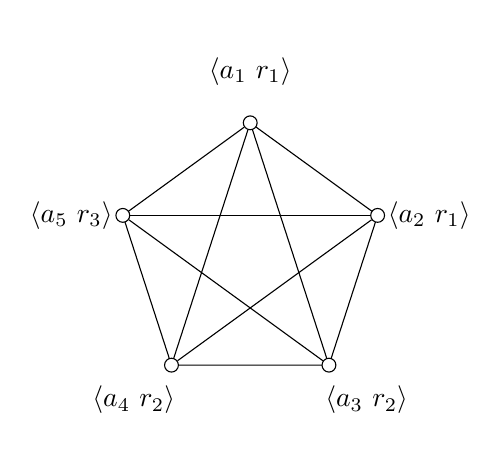
\begin{tikzpicture}
      \tikzstyle{every node}=[draw,circle,fill=white,minimum size=5pt,
			      inner sep=0pt]
      \draw (0,0) 	 node (agent1) [label=90:$\LD a_1\ r_1 \RD$] {}
	  -- ++(-36:2.0cm)   node (agent2) [label=right:$\LD a_2\ r_1 \RD$] {}
	  -- ++(-108:2.0cm) node (agent3) [label=-30:$\LD a_3\ r_2 \RD$] {}
	  -- ++(-180:2.0cm) node (agent4) [label=210:$\LD a_4\ r_2 \RD$] {}
	  -- ++(108:2.0cm) node (agent5) [label=left:$\LD a_5\ r_3 \RD$] {}
	  -- (agent1);
      \draw (agent1) -- (agent3);
      \draw (agent1) -- (agent4);
      \draw (agent2) -- (agent4);
      \draw (agent2) -- (agent5);
      \draw (agent3) -- (agent5);
  \end{tikzpicture}
  \label{subfig:fully_connected}
}\ \
\subfloat[Ring ($O_{r}$)]{
  \begin{tikzpicture}
      \tikzstyle{every node}=[draw,circle,fill=white,minimum size=5pt,
			      inner sep=0pt]
      \draw (0,0) 	 node (agent1) [label=90:$\LD a_1\ r_1 \RD$] {}
	  -- ++(-36:2.0cm)   node (agent2) [label=right:$\LD a_2\ r_2 \RD$] {}
	  -- ++(-108:2.0cm) node (agent3) [label=-30:$\LD a_3\ r_1 \RD$] {}
	  -- ++(-180:2.0cm) node (agent4) [label=210:$\LD a_4\ r_2 \RD$] {}
	  -- ++(108:2.0cm) node (agent5) [label=left:$\LD a_5\ r_3 \RD$] {}
	  -- (agent1);
  \end{tikzpicture}
  \label{subfig:ring}
}
\subfloat[Star ($O_{s}$)]{
  \begin{tikzpicture}
      \tikzstyle{every node}=[draw,circle,fill=white,minimum size=5pt,
			      inner sep=0pt]
      \draw (0,0) 	 node (agent1) [label=90:$\LD a_1\ r_1 \RD$] {}
	  -- ++(-36:2.0cm)   node (agent2) [label=right:$\LD a_2\ r_2 \RD$] {}
	   ++(-108:2.0cm) node (agent3) [label=-30:$\LD a_3\ r_2 \RD$] {}
	   ++(-180:2.0cm) node (agent4) [label=210:$\LD a_4\ r_3 \RD$] {}
	   ++(108:2.0cm) node (agent5) [label=left:$\LD a_5\ r_3 \RD$] {}
	  -- (agent1);
      \draw (agent1) -- (agent3);
      \draw (agent1) -- (agent4);
  \end{tikzpicture}
  \label{subfig:star}
}\ \
\subfloat[Isolated agent ($O_{ia}$)]{
  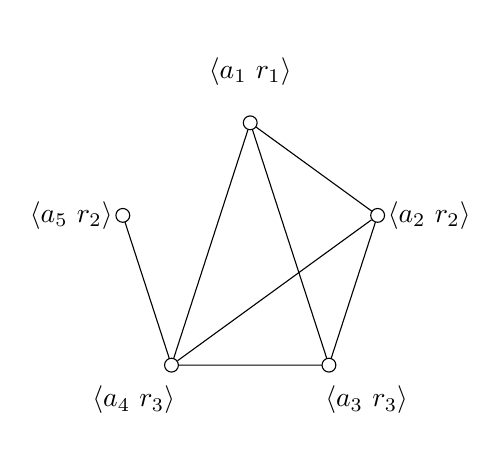
\begin{tikzpicture}
      \tikzstyle{every node}=[draw,circle,fill=white,minimum size=5pt,
			      inner sep=0pt]
      \draw (0,0) 	 node (agent1) [label=90:$\LD a_1\ r_1 \RD$] {}
	  -- ++(-36:2.0cm)   node (agent2) [label=right:$\LD a_2\ r_2 \RD$] {}
	  -- ++(-108:2.0cm) node (agent3) [label=-30:$\LD a_3\ r_3 \RD$] {}
	  -- ++(-180:2.0cm) node (agent4) [label=210:$\LD a_4\ r_3 \RD$] {}
	  -- ++(108:2.0cm) node (agent5) [label=left:$\LD a_5\ r_2 \RD$] {};
      \draw (agent1) -- (agent3);
      \draw (agent1) -- (agent4);
      \draw (agent2) -- (agent4);
  \end{tikzpicture}
  \label{subfig:isolated}
}}
\caption{Experimental configurations of the agent organisations with optimal resource allocation (see Tab.~\ref{tab:optimal_r}). In parentheses is the abbreviation that we will use to refer to the organisation throughout this paper.}
\label{fig:network_configurations}
\end{figure}


\section{Experimental Results}
\label{sec:results}
\vspace{-10pt}
In this section, we present results obtained using three models: DTMC, MDP, and STPG. Tab.~\ref{tab:model_sizes} compares model construction information for different sizes of fully connected agent organisations\footnote{We choose a fully connected agent organisation because it produces the largest models.}. All experiments are performed on a 2.8GHz Intel Core 2 PC, 4Gb of RAM running the Fedora Core 13 operating system. Nondeterministic models (MDPs/STPGs) have a smaller state space because agent choices do not have to be resolved at the model construction stage. However, the model checking is generally more time consuming for MDPs and STPGs than for DTMCs. The time needed for model checking is in the range of 5-240 seconds.

\begin{table}
\centering
\subfloat[DTMC]{
\begin{tabular}{ | l | l | l | l |}
    \hline
    Agents & States & Transitions & Constr. Time (s) \\ \hline
    2 & 1865 & 2256 & 0.1  \\ \hline
    3 & 17041 & 20904 & 0.3 \\ \hline
    4 & 184753 & 226736 & 3.4 \\ \hline
    5 & 2366305 & 2893536 & 74.4 \\ \hline
    6 & 35058241 & 42638400 & 2916.2 \\ \hline
\end{tabular}
}
\subfloat[MDP and STPG]{
 \begin{tabular}{ | l | l | l | l |}
    \hline
    Agents & States & Transitions & Constr. Time (s) \\ \hline
    2 & 1405 & 1846 & 0.1  \\ \hline
    3 & 9721 & 12474 & 0.2 \\ \hline
    4 & 76865 & 96664 & 1.1 \\ \hline
    5 & 731233 & 907992 & 5.1 \\ \hline
    6 & 8155873 & 10040112 & 29.7 \\ \hline
\end{tabular}
}
\caption{Model comparison for different numbers of agents in a fully connected agent organisation for the offline version of Alg.~\ref{alg:join_team_org}.}
\label{tab:model_sizes}
\end{table}
\vspace{-20pt}
As mentioned in Sec.~\ref{subsec:exp_set}, for each topology from Fig.~\ref{fig:network_configurations} we obtain optimal resource allocations using probabilistic model checking on the DTMC model of the offline version of the algorithm (see Alg.~\ref{alg:main_process} and Alg.~\ref{alg:join_team_org}). The following PRISM temporal logic queries are used to compute the expected rewards of the agent organisation under a particular resource allocation:
\vspace{-3pt}
\begin{itemize}
 \item ${\tt R}_{=?}^{W_{j}}[\,\Diamond\,\mathit{finished}\,]$ -
``what is the expected total reward  $W_j$ ($j\in\{1,2\}$) of an agent organisation when execution terminates?'',
\end{itemize}
\vspace{-5pt}
After obtaining the expected rewards for all possible resource allocations, we selected the with the highest expected reward. The results are summarised in Tab.~\ref{tab:optimal_r}.

\vspace{-5mm}

\begin{table}[H]
 \centering
 \begin{tabular}{ | l | l | l | l |}
    \hline
    Organisation $O$ & Additional constraints & Example $\LD R_{a_1}R_{a_2}R_{a_3}R_{a_4}R_{a_5}\RD$ \\ \hline
    $O_{\mathit{fc}}$ & - & $R_A=\LD \{r_1\}\{r_1\}\{r_2\}\{r_2\}\{r_3\}\RD$  \\ \hline
    $O_r$ & $R_{a_1}\neq R_{a_5} \wedge \forall i < 5 . R_{a_i} \neq  R_{a_{i+1}} $ & $R_A=\LD \{r_1\}\{r_2\}\{r_1\}\{r_2\}\{r_3\}\RD$  \\ \hline
    $O_s$ & $R_{a_1}=\{r\} \wedge \forall i > 1 . r \notin R_{a_i} $  & $R_A=\LD \{r_1\}\{r_2\}\{r_2\}\{r_3\}\{r_3\}\RD$  \\ \hline
    $O_{ia}$ & $R_{a_5}=\{r\} \wedge \exists i < 4 . r \in R_{a_i} $ & $R_A=\LD \{r_1\}\{r_2\}\{r_3\}\{r_3\}\{r_2\}\RD$  \\ \hline
\end{tabular}
\caption{Optimal resource allocations with respect to rewards defined in Eqn. \eqref{eq:w1organisation}. %and \ref{eq:w2organisation}.
All satisfy the constraint $\forall i. |R_{a_i}|=1 \wedge   \forall i.1 \le|\{ R_{a_j} : r_i \in R_{a_j} (1 \le j \le 5 )\}|\le 2$.}
\label{tab:optimal_r}
\end{table}
\vspace{-30pt}
Note that the resource allocations given in Tab.~\ref{tab:optimal_r}, column ``Example" will be used for all future experiments and are shown in Fig.~\ref{fig:network_configurations}. We have decided to fix resource allocations in this way as it allows us to show how model-checking techniques can be used to improve performance of the algorithm by synthesising strategies (see discussion of MDP results in Sec.~\ref{subsec:MDP}).
%\clearpage

\subsection{DTMC Analysis}
\label{subsection:DTMC}
\vspace{-10pt}
In this section, we present the results for model checking the DTMC model of Alg.~\ref{alg:join_team_org} for experimental agent organisations from Fig.~\ref{fig:network_configurations}, as well as offline and online versions of the algorithm (see Alg.~\ref{alg:main_process} for details).

\vspace{-10mm}

\begin{table} [H]
\subfloat[Offline. $W_1$ reward structure.]{
 \begin{tabular}{ | l | l | l | l | l |}
    \hline
    $O$ & $W_1(O)$ & $\min_{a \in A}W_1(a)$ & $\max_{a \in A}W_1(a)$ \\ \hline
    $O_{\mathit{fc}}$ & 2.54906 & 0.44958 & 0.75073   \\ \hline
    $O_r$  & 2.30359 & 0.35494 & 0.63985 \\ \hline
    $O_s$  & 1.87278 & 0.28677 & 0.72568  \\ \hline
    $O_{ia}$  & 2.38529 & 0.28867 & 0.68769  \\ \hline
\end{tabular}
}
\subfloat[Offline. $W_2$ reward structure.]{
 \begin{tabular}{ | l | l | l | l |}
    \hline
    $O$ & $W_2(O)$ & $\min_{a \in A}W_2(a)$ & $\max_{a \in A}W_2(a)$ \\ \hline
    $O_{\mathit{fc}}$ & 1.49125 & 0.26721 & 0.42238 \\ \hline
    $O_r$ & 1.42923 & 0.23531 & 0.38625 \\ \hline
    $O_s$ & 1.16649 & 0.18582 & 0.42321  \\ \hline
    $O_{ia}$ & 1.43599 & 0.20621 & 0.39907  \\ \hline
\end{tabular}
}
\vspace{-8pt}
\subfloat[Online. $W_1$ reward structure.]{
 \begin{tabular}{ | l | l | l | l | l |}
    \hline
    $O$ & $W_1(O)$ & $\min_{a \in A}W_1(a)$ & $\max_{a \in A}W_1(a)$ \\ \hline
    $O_{\mathit{fc}}$ & 3.53645 & 0.64101 & 0.97239   \\ \hline
    $O_r$  & 3.48638 & 0.55089 & 0.91190 \\ \hline
    $O_s$  & 2.52500 & 0.41934 & 0.84761  \\ \hline
    $O_{ia}$  & 3.37359 & 0.41186 & 0.93601  \\ \hline
\end{tabular}
}
\subfloat[Online. $W_2$ reward structure.]{
 \begin{tabular}{ | l | l | l | l |}
    \hline
    $O$ & $W_2(O)$ & $\min_{a \in A}W_2(a)$ & $\max_{a \in A}W_2(a)$ \\ \hline
    $O_{\mathit{fc}}$ & 1.29743 & 0.24247 & 0.32657 \\ \hline
    $O_r$ & 1.31882 & 0.23157 & 0.31297 \\ \hline
    $O_s$ & 0.94404 & 0.16060 & 0.30158  \\ \hline
    $O_{ia}$ & 1.25560 & 0.17970 & 0.31990  \\ \hline
\end{tabular}
}
\caption{Model checking results for agent organisations from Fig.~\ref{fig:network_configurations} with optimal resource allocations from Tab.~\ref{tab:optimal_r} for offline and online versions of Alg.~\ref{alg:main_process}. Tables also show largest and smallest individual agent rewards. }
\label{tab:dtmc_results}
\end{table}
\vspace{-25pt}
Tab.~\ref{tab:dtmc_results} shows the results obtained for the expected rewards of agent organisations in different settings, namely, using $W_1$ and $W_2$ reward structures (see Eqn. \eqref{eq:w1organisation} %and \ref{eq:w2organisation}
for organisations and Eqn.~\eqref{eq:w1agent} and Eqn.~\eqref{eq:w2agent} for individual agents), and offline and online versions of Alg.~\ref{alg:join_team_org}. The following PRISM temporal logic queries were used to obtain the results:
\vspace{-5pt}
\begin{itemize}
 \item ${\tt R}_{=?}^{W_{j}(O)}[\,\Diamond\,\mathit{finished}\,]$ -
``what is the expected total reward $W_j$ ($j\in\{1,2\}$)?'',
 \item ${\tt R}_{=?}^{W_{j}(O)}[\,\Diamond\,(\mathit{finished} \wedge a_i {\in} \bar{M}) \,]$ -
``what is the expected reward $W_j$ ($j\in\{1,2\}$) for agent $a_i$ ($i\in\{1,2,3,4,5\}$)?''
\end{itemize}
\vspace{-5pt}
As can be seen in Tab.~\ref{tab:dtmc_results}, agents organised in $O_s$ have the worst expected rewards in all settings, and also the largest disparity between the worst and best performing individual agents. Both of these characteristics are not surprising because agent $a_1$, which is placed in the middle, is most likely to be in a winning team, whereas the others do not have any choice but to join the team with $a_1$. Organisation $O_{ia}$, which has one isolated agent, shows a smaller differences between the worst and the best performing agents, but this is only because the performance of the ``best'' agents is lower, whereas the ``worst'' agent's performance is very close to that of $O_s$.

Fig.~\ref{fig:bar_chart_dtmc} compares total rewards of all organisations in offline and online settings. It can be seen that a fully connected organisation $O_{\mathit{fc}}$ has the best overall performance in all but the online version using the $W_2$ reward structure, where it is outperformed by $O_r$. It is interesting to note that a more significant difference between $O_{\mathit{fc}}$ and $O_{ia}$ only emerges when moving to the online setting. This shows that having one agent which is isolated does not affect the ability of the organisation to efficiently respond to the generated tasks, but impacts its chances to organise before the tasks are generated. This is where the advantages of $O_r$ emerge: in the online setting, it not only starts outperforming $O_{ia}$ with respect to overall performance and disparity, but gets very close to the performance of $O_{\mathit{fc}}$ using the $W_1$ reward structure, and produces a better total $W_2$ reward while keeping similar disparity levels.

\vspace{-10mm}
\begin{figure}[H]
\centering
\scalebox{0.8}{
\subfloat[Reward $W_1(O)$.]{
  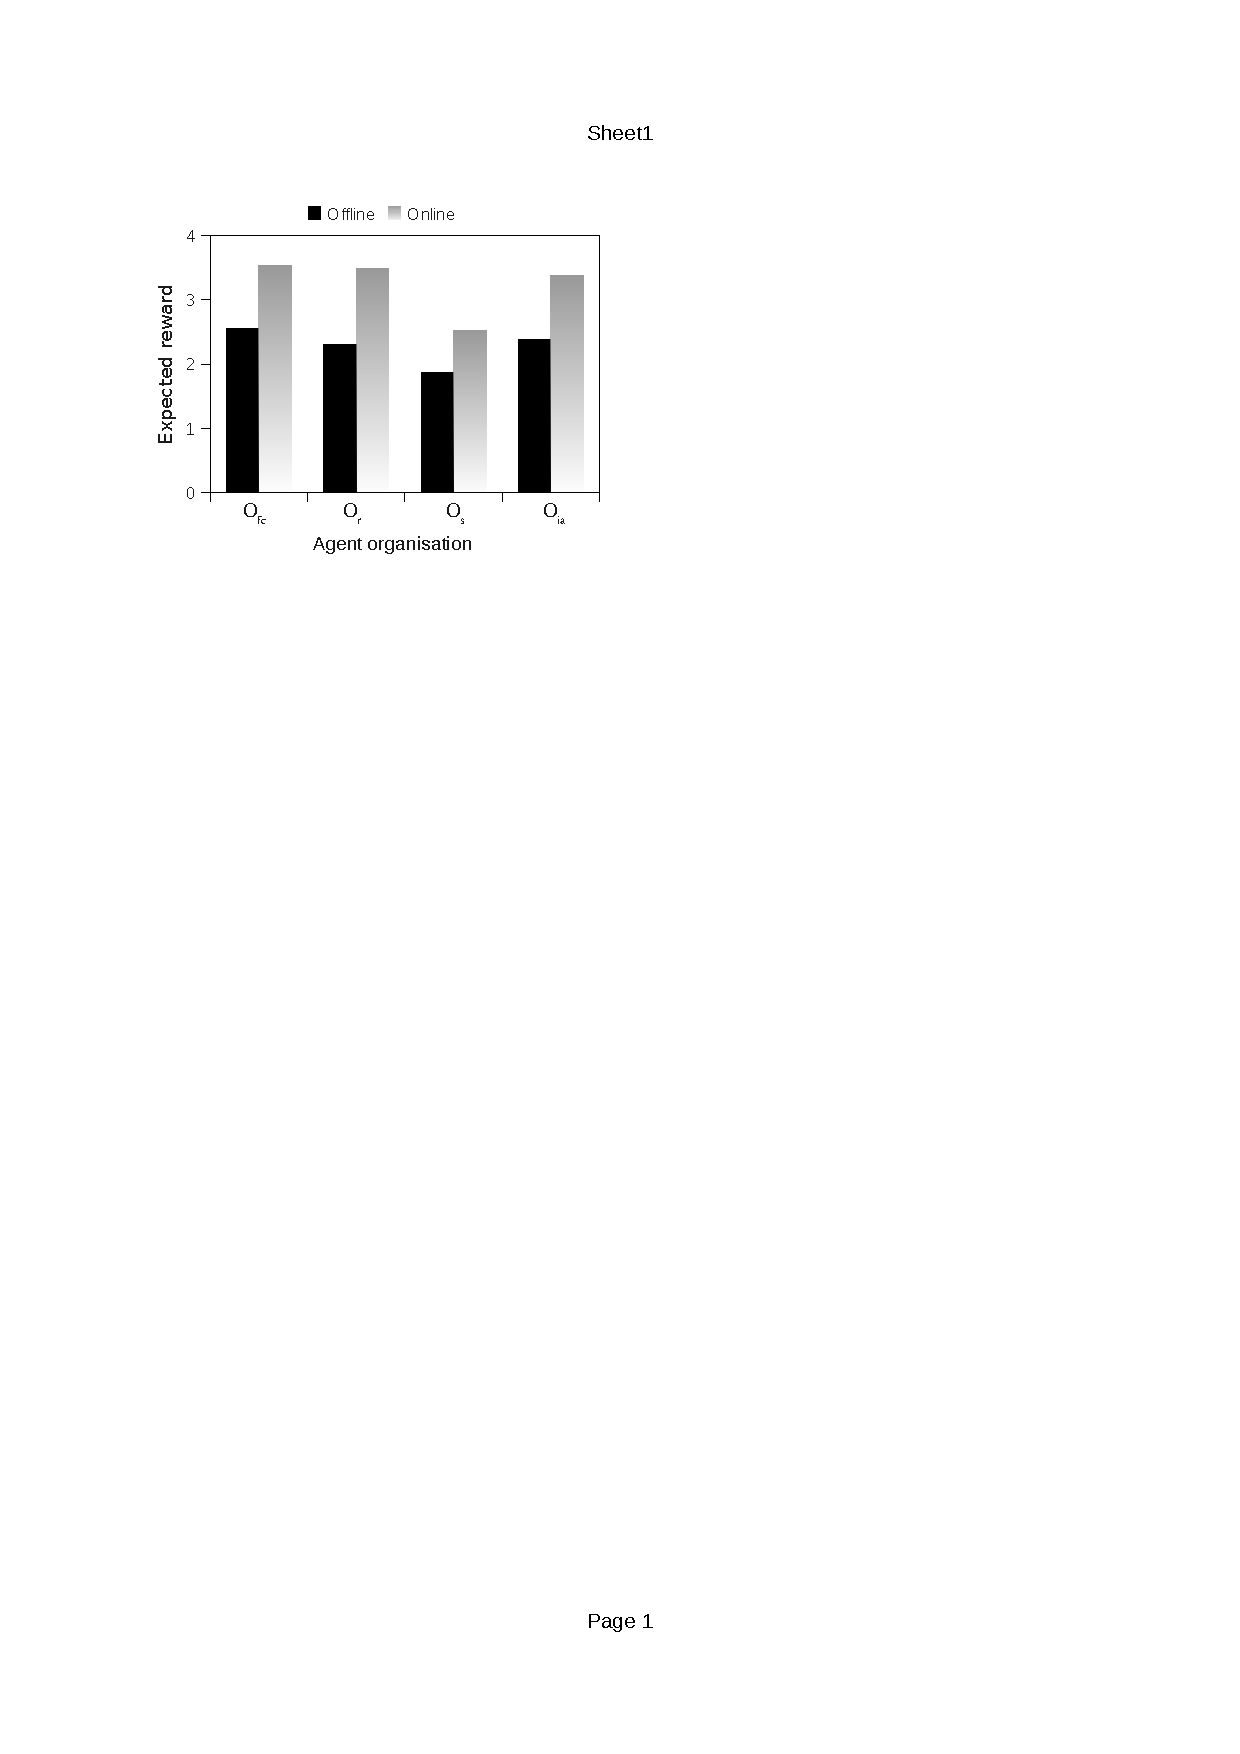
\includegraphics[clip=true, trim=75 570 305 90, scale=0.77]{images/w1_dtmc}
}
\subfloat[Reward $W_2(O)$.]{
  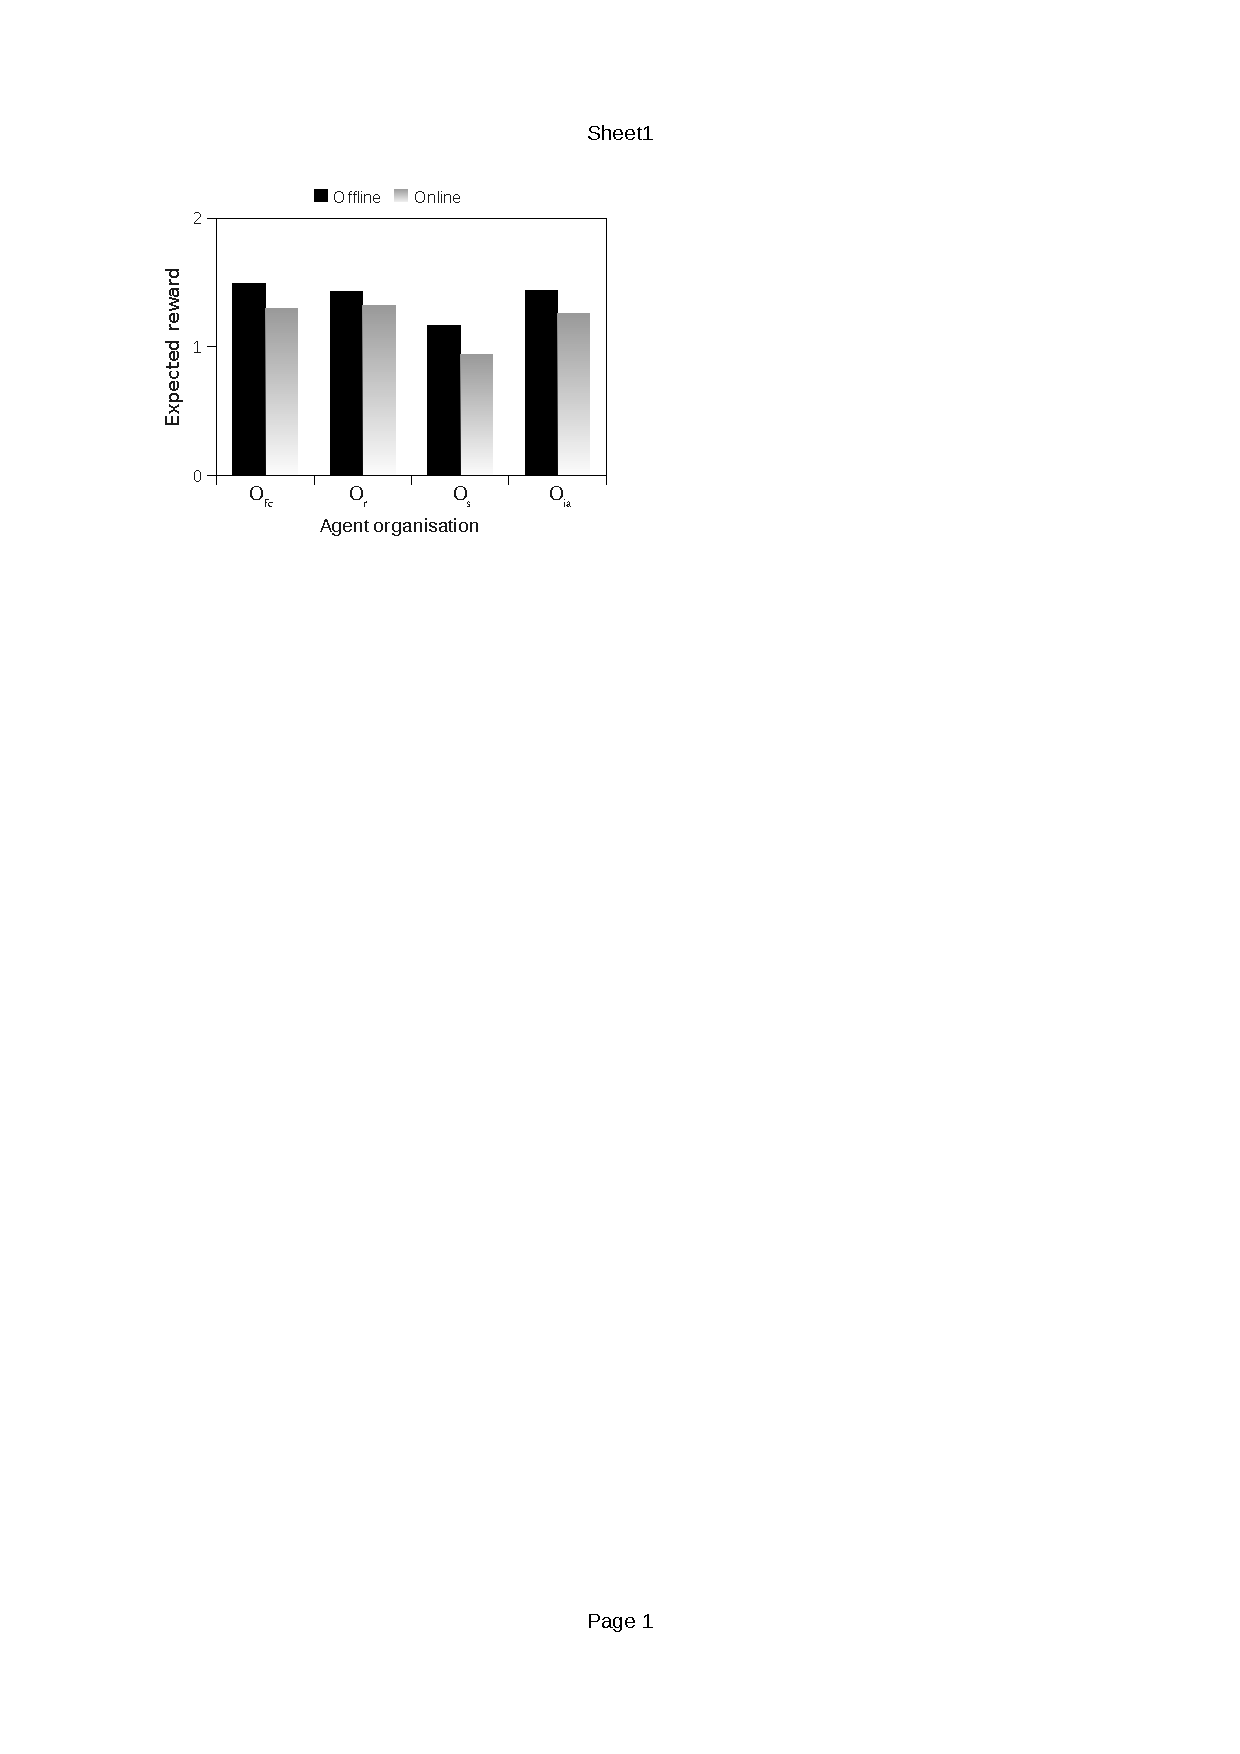
\includegraphics[clip=true, trim=70 579 300 90, scale=0.77]{images/w2_dtmc}
}}
\vspace{-10pt}
\caption{Expected rewards for agent organisations when using online and offline (see Alg.~\ref{alg:main_process}) versions of Alg.~\ref{alg:join_team_org}.}
\label{fig:bar_chart_dtmc}
\end{figure}
\vspace{-8mm}


An attentive reader would have noticed that the online version produces larger expected $W_1$, but smaller expected $W_2$ rewards. This observation shows that, in an online version, the algorithm organises agents into teams which increases the expectation for more agents to be in a successful team, but that this decreases the expected total number of tasks completed. These are summarised in Tab.~\ref{tab:task_compl_dtmc} where the task completion probabilities are presented. The following PRISM temporal logic queries were used to find the probabilities:
\vspace{-5pt}
\begin{itemize}
 \item ${\tt P}_{=?}[\,\Diamond\,T_{j} \mathit{\ completed}\,]$ -
``what is the expected probability to complete  task $T_j$ ($j\in\{1,2\}$)?'',
 \item ${\tt P}_{=?}[\,\Diamond\,(T_{1} \wedge T_2 \mathit{\ completed})\,]$ -
``what is the expected probability to complete  both tasks $T_1$ and $T_2$?'',
\end{itemize}
\vspace{-30pt}

\begin{table}[H]
 \centering
\subfloat[Offline]{
 \begin{tabular}{ | l | l | l | l |}
    \hline
    $O$ & $T_1$ compl. & $T_2$ compl. & $T_1$ and $T_2$ compl. \\ \hline
    $O_{\mathit{fc}}$ & 0.74562 & 0.74562 & 0.49596  \\ \hline
    $O_r$ & 0.71461 & 0.71461 & 0.47062 \\ \hline
    $O_s$ & 0.58324 & 0.58324 & 0.23639 \\ \hline
    $O_{ia}$ & 0.71799 & 0.71799 & 0.44839 \\ \hline
\end{tabular}
}
\subfloat[Online]{
 \begin{tabular}{ | l | l | l | l |}
    \hline
    $O$ & $T_1$ compl. & $T_2$ compl. & $T_1$ and $T_2$ compl. \\ \hline
    $O_{\mathit{fc}}$ & 0.64871 & 0.64871 & 0.31320  \\ \hline
    $O_r$ & 0.65941 & 0.65941 & 0.36712 \\ \hline
    $O_s$ & 0.47202 & 0.47202 & 0.07465 \\ \hline
    $O_{ia}$ & 0.62780 & 0.62780 & 0.29270 \\ \hline
\end{tabular}
}
\caption{Task completion probabilities for optimal agent organisations using Alg.~\ref{alg:join_team_org}'s offline and online versions (see Alg.~\ref{alg:main_process}).}
\label{tab:task_compl_dtmc}
\end{table}
\vspace{-30pt}
%Let us note that the strategy of an agent does not change when switching from the offline to online setting, but it is the same strategy and the removal of constraint that the agent can only join a team for a task that it has the required skill for (which is obviously not known before the task is advertised) that results more agents joining teams.

Using formal analysis for DTMCs, we produced \emph{exact} values of expectations for properties of the system (task completion probabilities and rewards were used as examples), so that even small differences between different organisations can be captured precisely. Also, we focused on one particular strategy defined in Alg. \ref{alg:join_team_org}, but the PRISM code can be adapted easily to analyse other strategies and reward structures. In the next section we will explore how the performance can be improved by changing the strategy of the agents so that they collaborate to optimise the performance of the organisation.
%\clearpage
\vspace{-10pt}
\subsection{MDP Analysis}
\label{subsec:MDP}
\vspace{-2pt}
In this section, we present the analysis of Alg.~\ref{alg:join_team_nondet}, which is modelled as an MDP. Using PRISM we find the maximum expected rewards and task completion probabilities for all agent organisations and compare the results with the strategy used in Alg.~\ref{alg:join_team_org}. Due to space limitations we do not present the actual strategies here.\footnote{The instructions on how to generate optimal strategies for MDPs can be found at:\\ {\scriptsize\url{http://www.prismmodelchecker.org/dev/manual/RunningPRISM/Adversaries.html}}}.

\vspace{-25pt}
\begin{table}
\centering
\subfloat[Offline]{
 \begin{tabular}{ | l | l | l | l |}
    \hline
    $O$ & $T_1$ compl. & $T_2$ compl. & $T_1$ and $T_2$ compl. \\ \hline
    $O_{\mathit{fc}}$ & 1.0 & 1.0 & 0.67346  \\ \hline
    $O_r$ & 1.0 & 1.0 & 0.67346  \\ \hline
    $O_s$ & 0.82857 & 0.82857 & 0.39183 \\ \hline
    $O_{ia}$ & 1.0 & 1.0 & 0.67346 \\ \hline
\end{tabular}
}
\subfloat[Online]{
 \begin{tabular}{ | l | l | l | l |}
    \hline
    $O$ & $T_1$ compl. & $T_2$ compl. & $T_1$ and $T_2$ compl. \\ \hline
    $O_{\mathit{fc}}$ & 1.0 & 1.0 & 0.42857  \\ \hline
    $O_r$ & 1.0 & 1.0 & 0.42857 \\ \hline
    $O_s$ & 0.88571 & 0.88571 & 0.12653 \\ \hline
    $O_{ia}$ & 1.0 & 1.0 & 0.42857 \\ \hline
\end{tabular}
}
\caption{Maximum task completion probabilities for optimal agent organisations using Alg.~\ref{alg:join_team_nondet}'s online and offline versions (see Alg.~\ref{alg:main_process}).}
\label{tab:mdp_probs}
\end{table}
\vspace{-25pt}
In Tab.~\ref{tab:mdp_probs} we can see the maximum expected task completion probabilities that can be achieved. All organisations except $O_s$ can ensure that at least one task is completed with probability $1.0$, no matter what the scheduling is. The following PRISM temporal logic queries were used to get the results:
\begin{itemize}
 \item ${\tt P}_{max=?}[\,\Diamond\,T_{j} \mathit{\ completed}\,]$ -
``what is the maximum expected probability to complete  task $T_j$ ($j\in\{1,2\}$)?'',
 \item ${\tt P}_{max=?}[\,\Diamond\,(T_{1} \wedge T_2 \mathit{\ completed})\,]$ -
``what is the maximum expected probability to complete  both tasks $T_1$ and $T_2$?''.
\end{itemize}

Tab.~\ref{tab:mdp_rewards} shows the maximum expected organisation rewards that can be achieved by all agents collaborating. It is not very difficult to see that $O_{\mathit{fc}}$, $O_r$ and $O_{ia}$ have the same maximum reward, no matter whether $W_1$/$W_2$ reward or online/offline version is taken. These outperform the star organization $O_s$ in all circumstances. The PRISM temporal logic queries used to find the rewards were the following:
\begin{itemize}
 \item ${\tt R}_{max=?}^{W_{j}}[\,\Diamond\,\mathit{finished}\,]$ -
``what is the maximum expected total reward $W_j$ ($j\in\{1,2\}$)?'',
 \item ${\tt R}_{max=?}^{W_{j}}[\,\Diamond\,(\mathit{finished} \,\wedge\, a_i {\in} \bar{M}) \,]$ -
``what is the maximum expected reward $W_j$ ($j\in\{1,2\}$) for agent $a_i$ ($i\in\{1,2,3,4,5\}$)?''
\end{itemize}

\vspace{-30pt}
\begin{table}[H]
\centering
\subfloat[Offline]{
 \begin{tabular}{ | l | l | l | l |}
    \hline
    $O$ & Max $W_1(O)$ & Max $W_2(O)$ \\ \hline
    $O_{\mathit{fc}}$ & 2.89795 & 1.67346   \\ \hline
    $O_r$ & 2.89795 & 1.67346  \\ \hline
    $O_s$ & 2.20816 & 1.35918  \\ \hline
    $O_{ia}$ & 2.89795 & 1.67346  \\ \hline
\end{tabular}
}
\subfloat[Online]{
 \begin{tabular}{ | l | l | l | l |}
    \hline
    $O$ & Max $W_1(O)$ & Max $W_2(O)$ \\ \hline
    $O_{\mathit{fc}}$ & 3.85714 & 1.42857   \\ \hline
    $O_r$ & 3.85714 & 1.42857  \\ \hline
    $O_s$ & 2.71428 & 1.02857  \\ \hline
    $O_{ia}$ & 3.85714 & 1.42857  \\ \hline
\end{tabular}
}
\vspace{-2pt}
\caption{Maximal rewards that can be achieved by agent organisations from Fig.~\ref{fig:network_configurations} using Alg.~\ref{alg:join_team_nondet}'s offline and online versions defined in Alg.~\ref{alg:main_process}.}
\label{tab:mdp_rewards}
\end{table}
\vspace{-32pt}

Fig.~\ref{fig:bar_chart_mdp} compares maximum expected rewards for Alg.~\ref{alg:join_team_org} which was analysed  in the previous section. More significant improvement can be obtained for the offline version for both rewards than for the online version. This result shows that there is more potential for collaboration for agents in the offline version. The small performance improvement for the online version suggests that the original strategy of Alg. \ref{alg:join_team_org} is close to optimal when teams are formed before tasks are advertised.


%
%
%
%It can be seen that a fully connected organisation $O_{\mathit{fc}}$ has the best overall performance in all but the online version using $W_2$ reward structure, where it is outperformed by organisation $O_r$ which arranged in a ring. It is interesting to see that a more significant difference between $O_{\mathit{fc}}$ and $O_{ia}$ only emerges when moving into algorithm's online setting, this shows that having one agent which is isolated does not affect the ability of the organisation to effciently respond to a generated tasks, but impacts its chances to organise before tasks are generated. And this where the advantages $O_r$ emerge, in online setting it not starts outperfoming $O_{ia}$ in respect with both overall performance and disparity, but gets very close to the performance of $O_{\mathit{fc}}$ using $W_1$ reward structure and produces a better total $W_2$ reward, while keeping disparity levels close.
\vspace{-10mm}
\begin{figure}[H]
\centering
\subfloat[Offline. Reward $W_1(O)$.]{
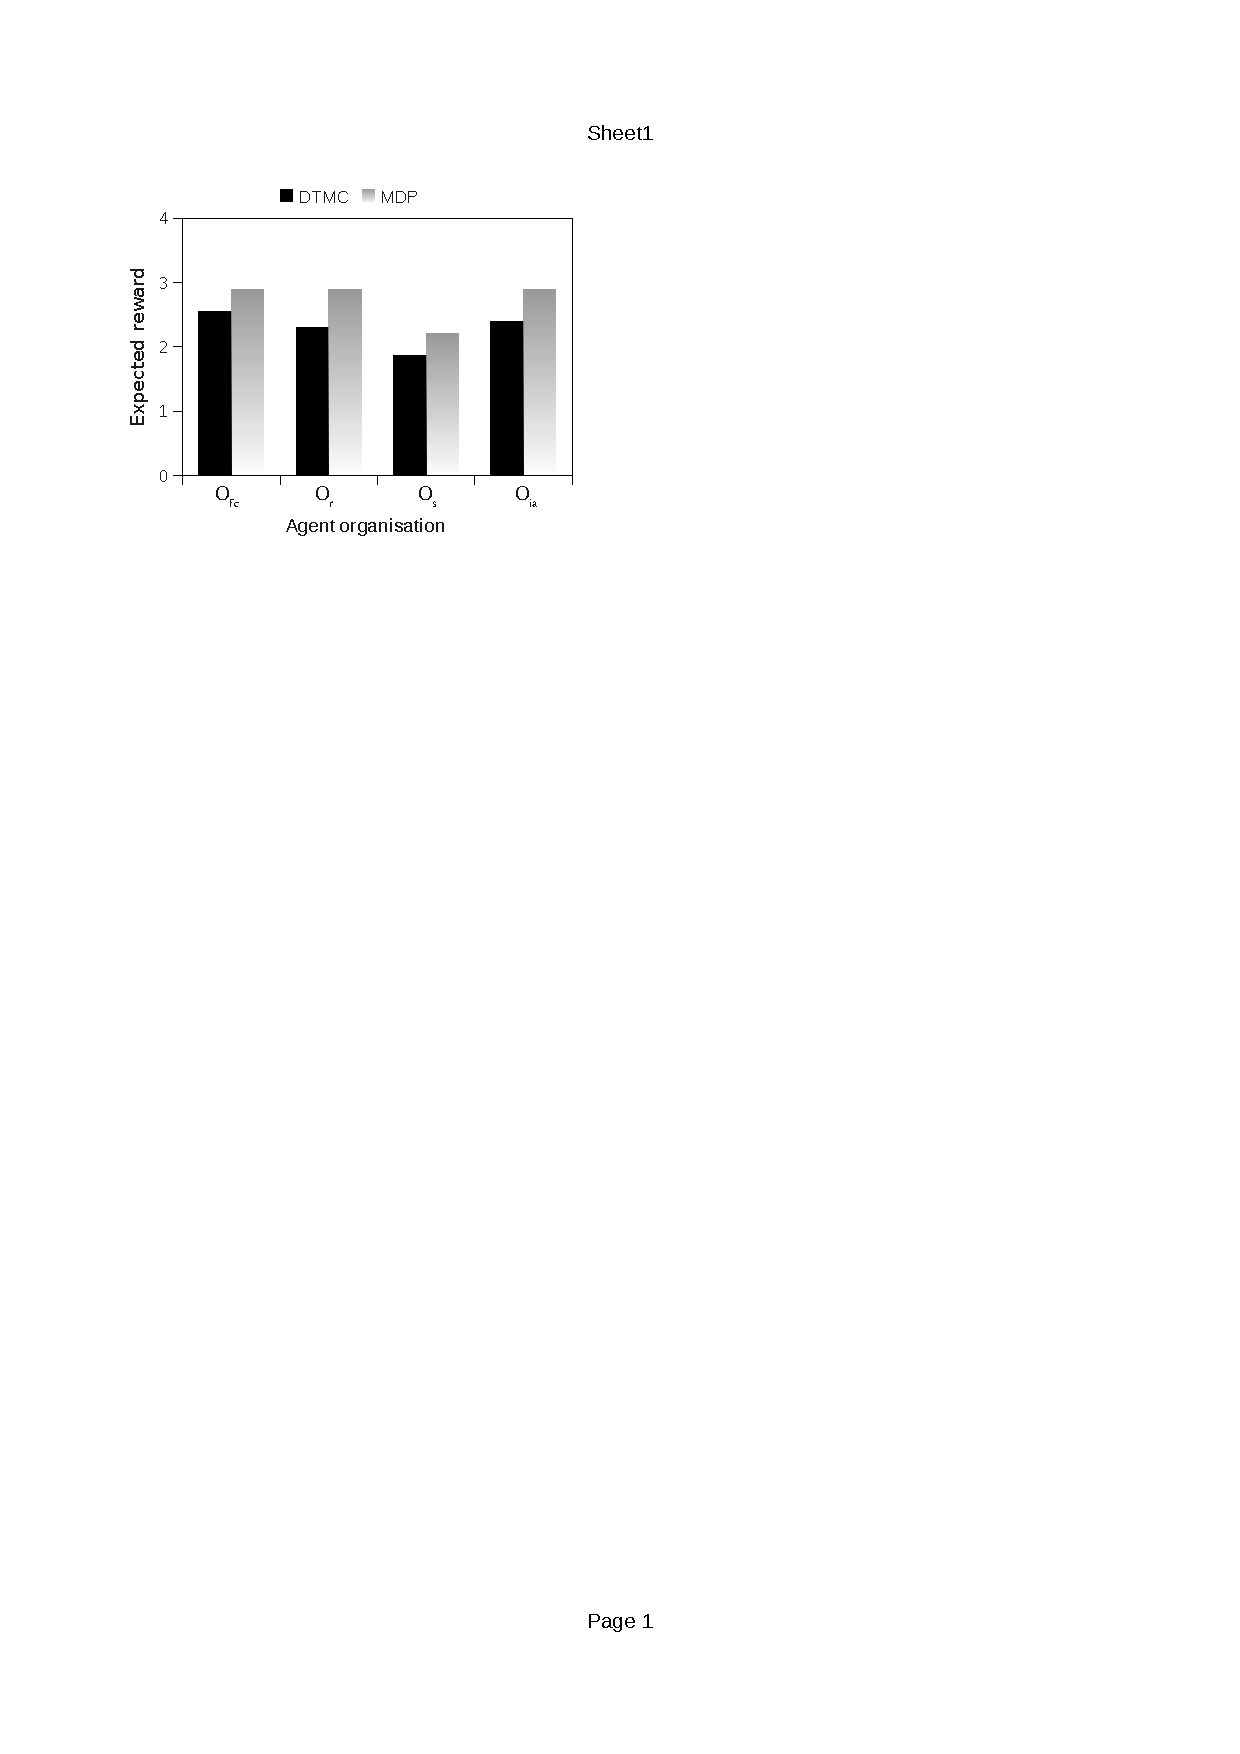
\includegraphics[clip=true, trim=60 580 320 90, scale=0.63]{images/w1_mdp_offline}
}
\subfloat[Online. Reward $W_1(O)$.]{
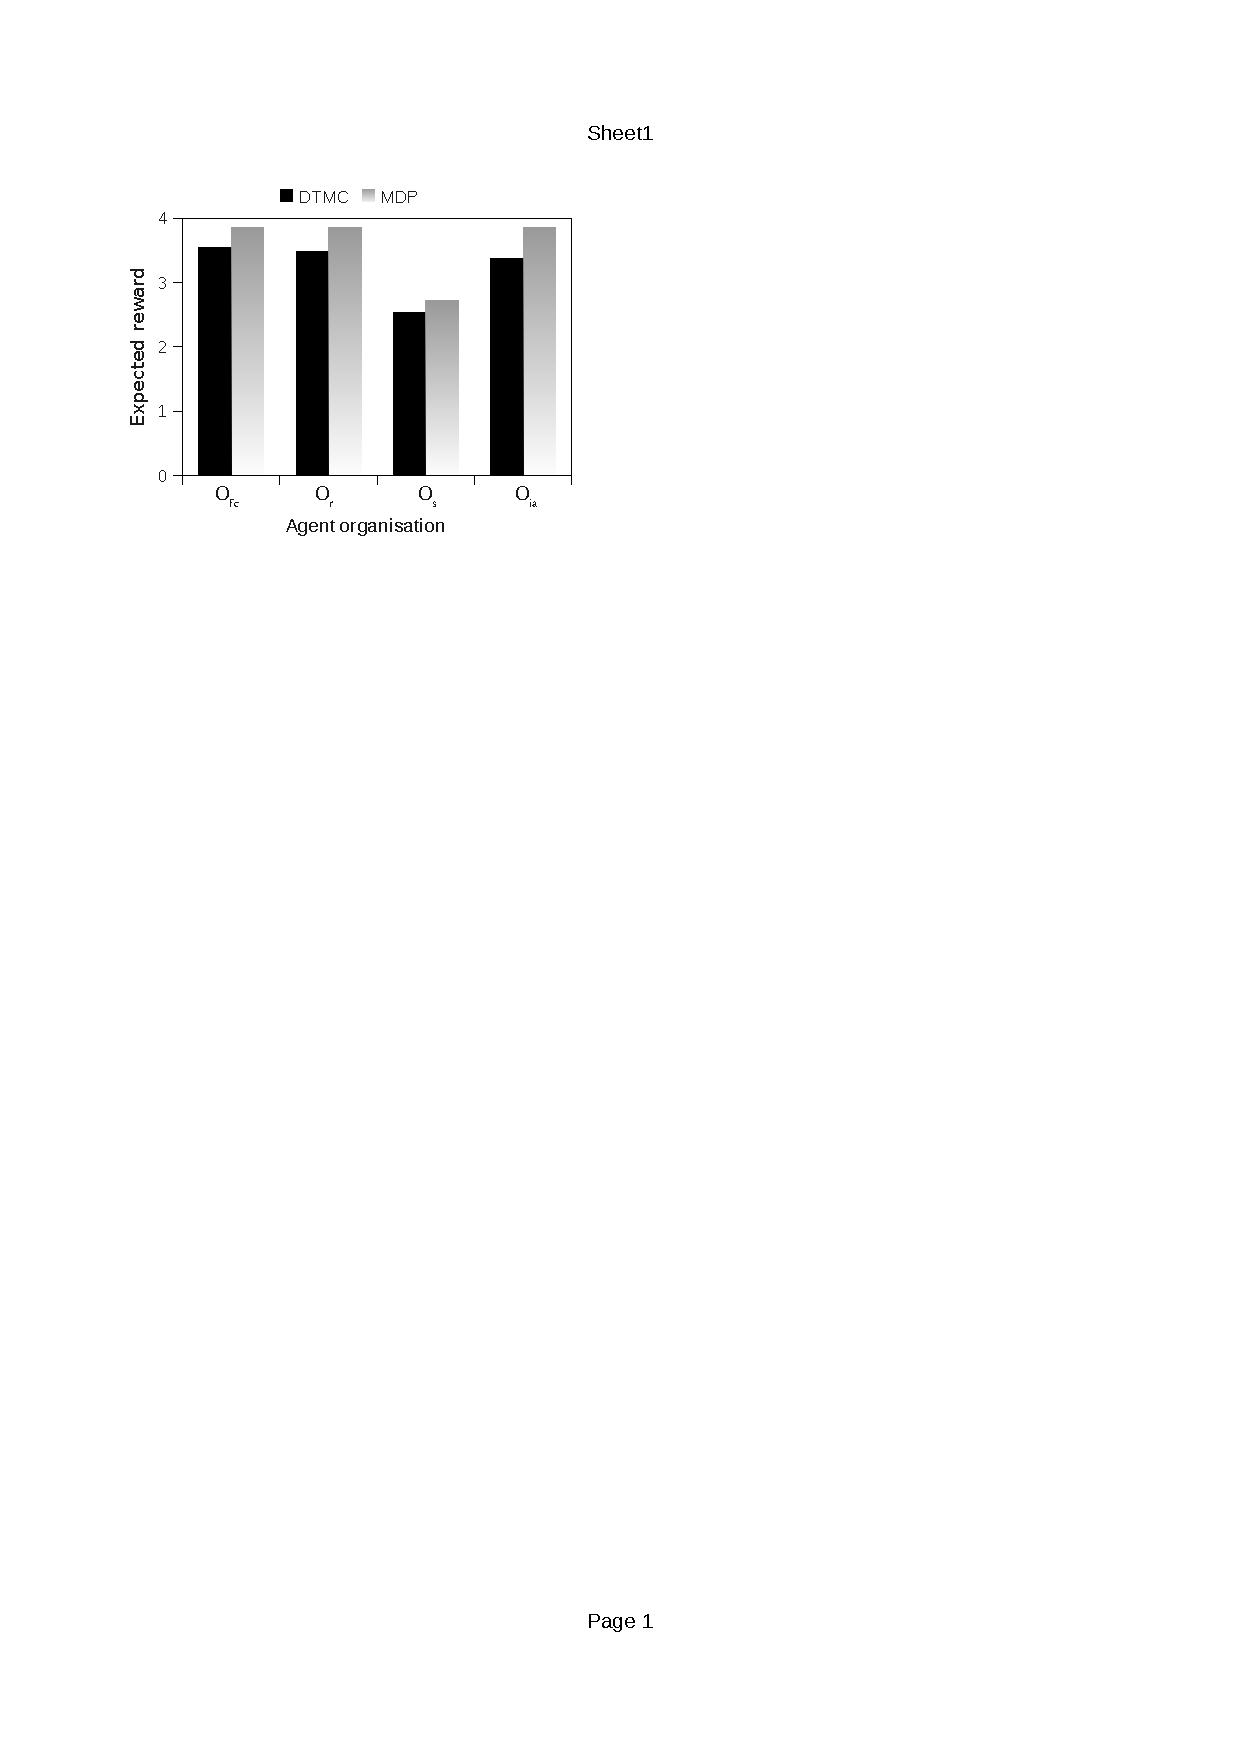
\includegraphics[clip=true, trim=57 580 320 90, scale=0.63]{images/w1_mdp_online}
}
\vspace{-13pt}
\subfloat[Offline. Reward $W_2(O)$.]{
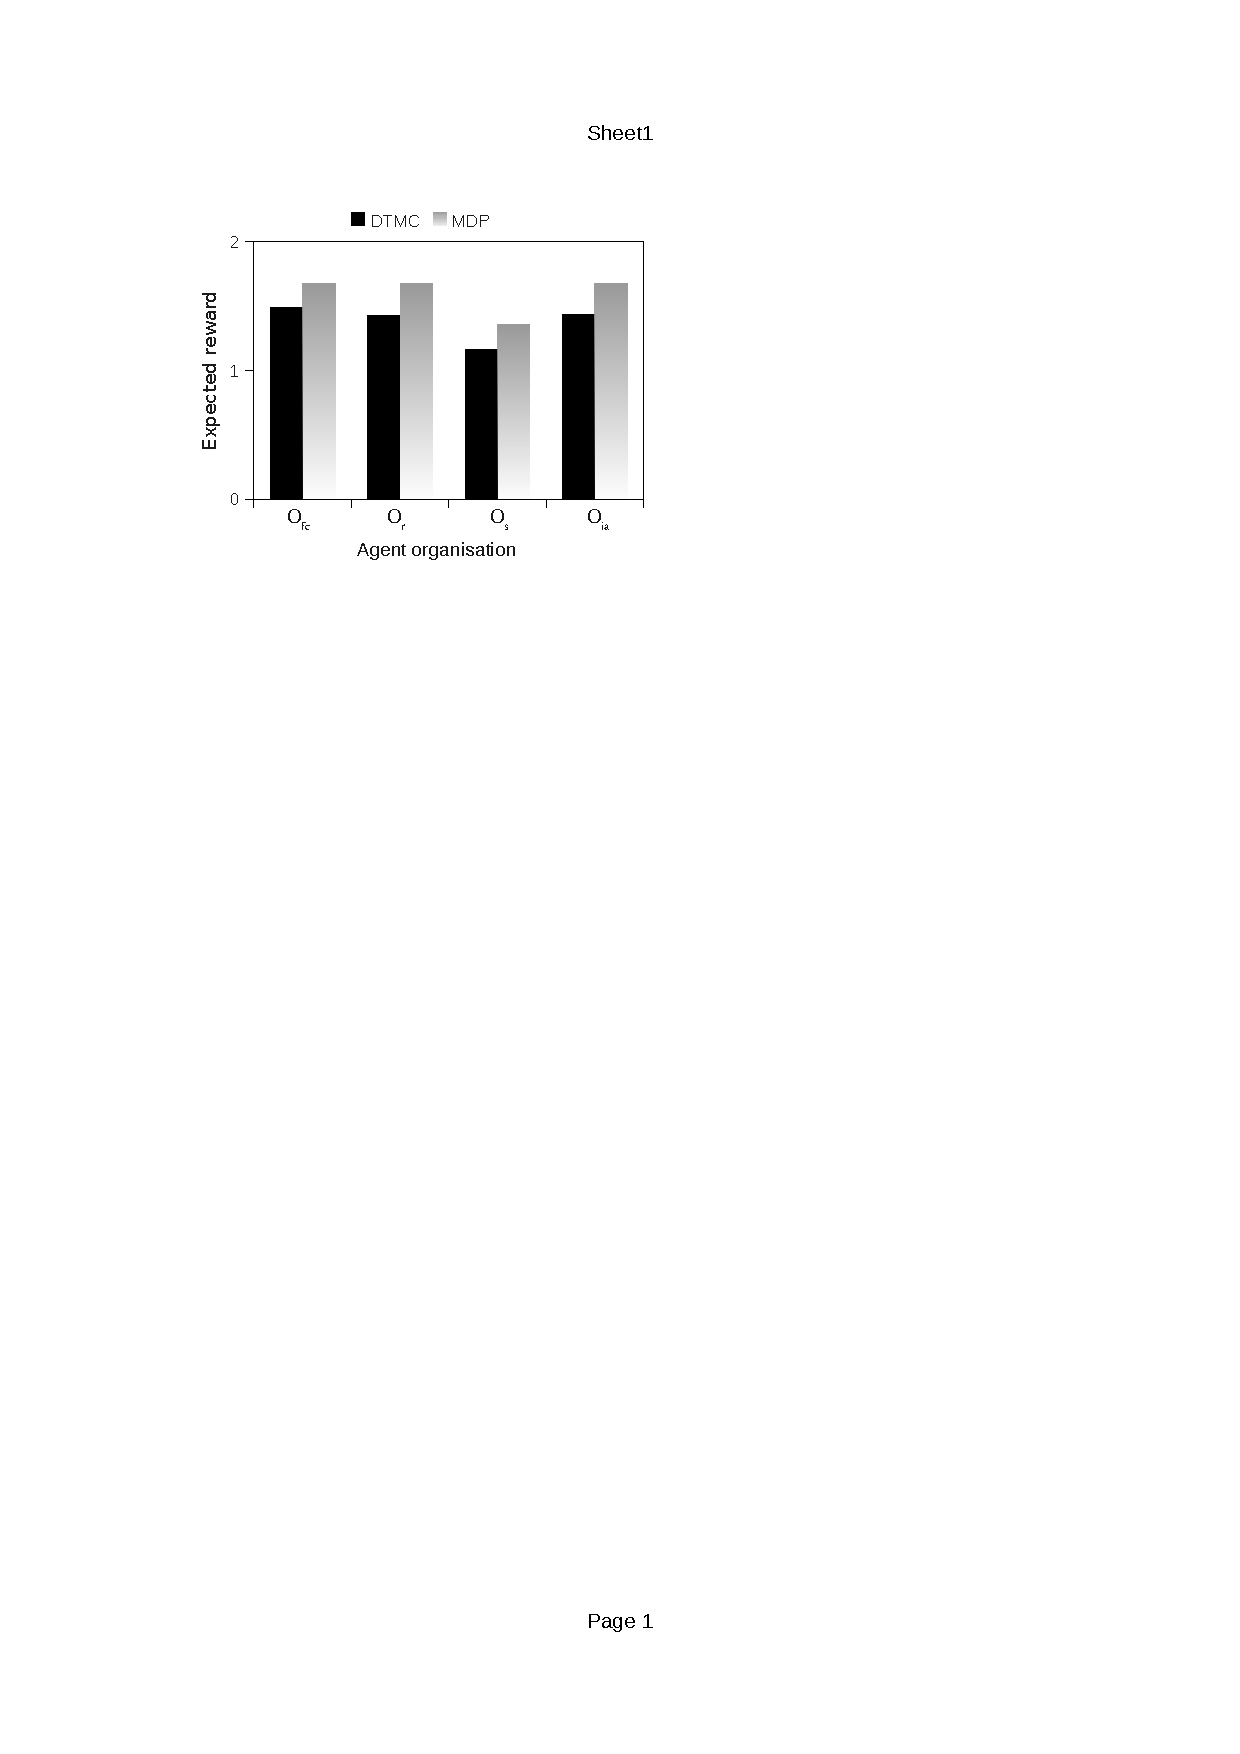
\includegraphics[clip=true, trim=94.5 570 280 100, scale=0.63]{images/w2_mdp_offline}
}
\subfloat[Online. Reward $W_2(O)$.]{
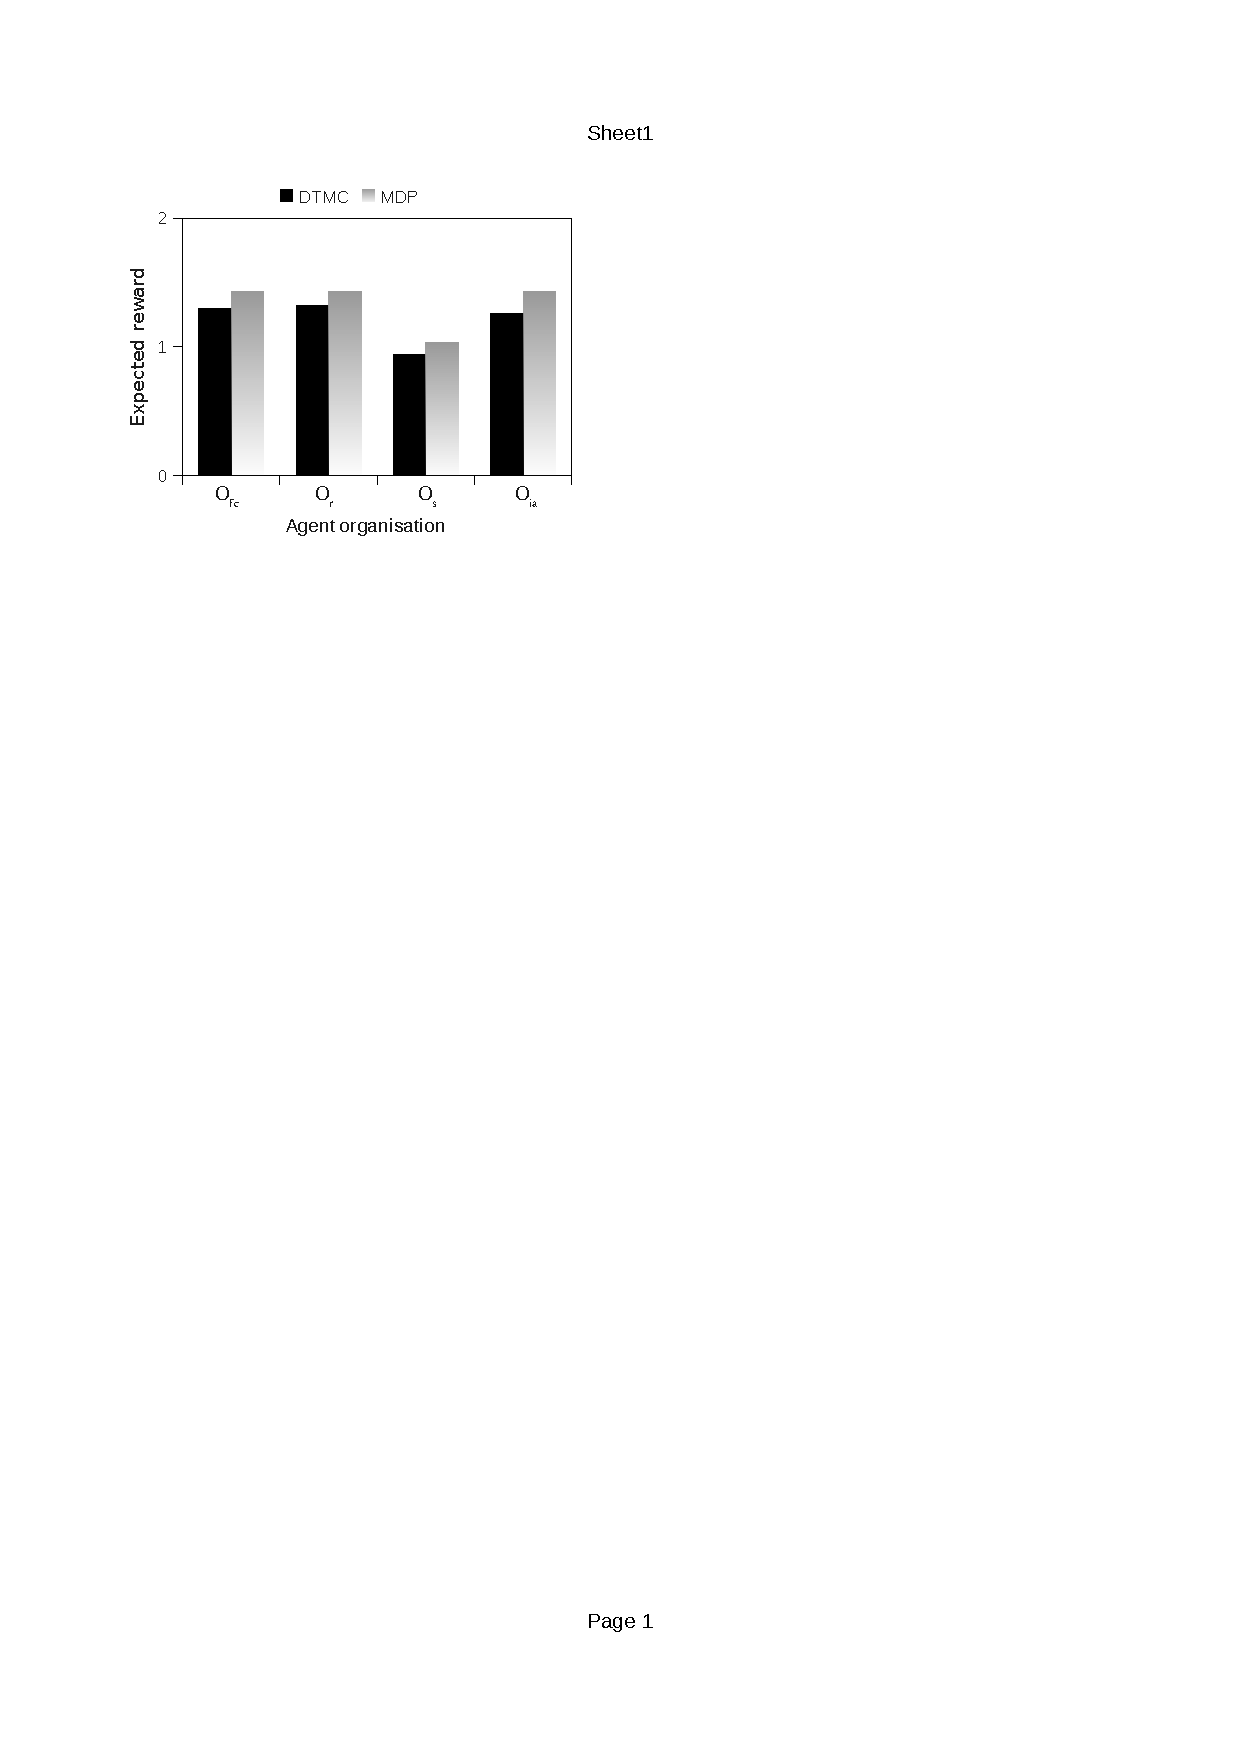
\includegraphics[clip=true, trim=63 581.5 320 80, scale=0.63]{images/w2_mdp_online}
}
\vspace{-10pt}
\caption{Bar charts comparing offline and online versions of Alg.~\ref{alg:join_team_org} analysed as a DTMC with the best-case performance of Alg.~\ref{alg:join_team_nondet} analysed as an MDP. }
\label{fig:bar_chart_mdp}
\end{figure}

\vspace{-22pt}


Using MDP model checking we have obtained the optimal strategy for the protocol and compared its performance to Alg.~\ref{alg:join_team_org}. It is worth noting that, even if the designer chooses not to implement this particular strategy, it still serves as a ``best-case'' benchmark for measuring other algorithms' performance. This analysis allows us to evaluate the effects of a fully collaborative behaviour of agents. However often only limited collaboration can be achieved (e.g. organisation containing hostile agents). In order to facilitate analysis of such systems, one has to go beyond MDPs. In the next section we show how STPGs can be used for this purpose.

\vspace{-10pt}
\subsection{STPG Analysis}
\label{subsec:STPG}
\vspace{-5pt}
In this section we focus on the analysis of Alg.~\ref{alg:join_team_nondet}, but, in contrast to the previous section,
we distinguish agents as either cooperative or hostile. This is naturally modelled as an STPG,
by considering each class of agents (cooperative or hostile) as a separate player.
%We refer to the collective cooperative agents as a \emph{coalition}.

We are mainly interested in finding the optimal coalition. In general,
a coalition $C\subseteq A$ is a subset of agents who cooperate to ensure certain goals irrespective of how the rest of the agents behave in the organization. We consider two criteria, i.e., the largest probability to accomplish tasks, and the largest reward ($W_1$ or $W_2$) achieved by the coalition. To this aim, we consider a slight extension of PCTL formulae with agent coalitions. The following formulae were used to obtain the results presented in this section:
\vspace{-5pt}
\begin{itemize}
 \item ${\tt P}_{max,min=?}[\,\Diamond\,T_{j} \mathit{\ completed}\,]$ -
``what is the maximum probability for coalition C to complete task $T_j$ ($j\in\{1,2\}$) when agents in $A\setminus C$ are hostile?'',
 \item ${\tt P}_{max,min=?}[\,\Diamond\,(T_{1} \wedge T_2 \mathit{\ completed})\,]$ -
``what is the maximum probability for coalition C to complete both tasks $T_1$ and $T_2$ when agents in $A\setminus C$ are hostile?'',
 \item ${\tt R}_{max,min=?}^{W_{j}}[\,\Diamond\,\mathit{finished}\,]$ -
``what is the maximum expected reward $W_j$ ($j\in\{1,2\}$) for coalition C when agents in $A\setminus C$ are hostile?'',
\end{itemize}
\vspace{-35pt}

\begin{figure}[H]
\ \ \ \ \ \ \ \ \ \ \ \subfloat[Offline. Reward $W_1(O)$.]{\label{fig:off_w1}
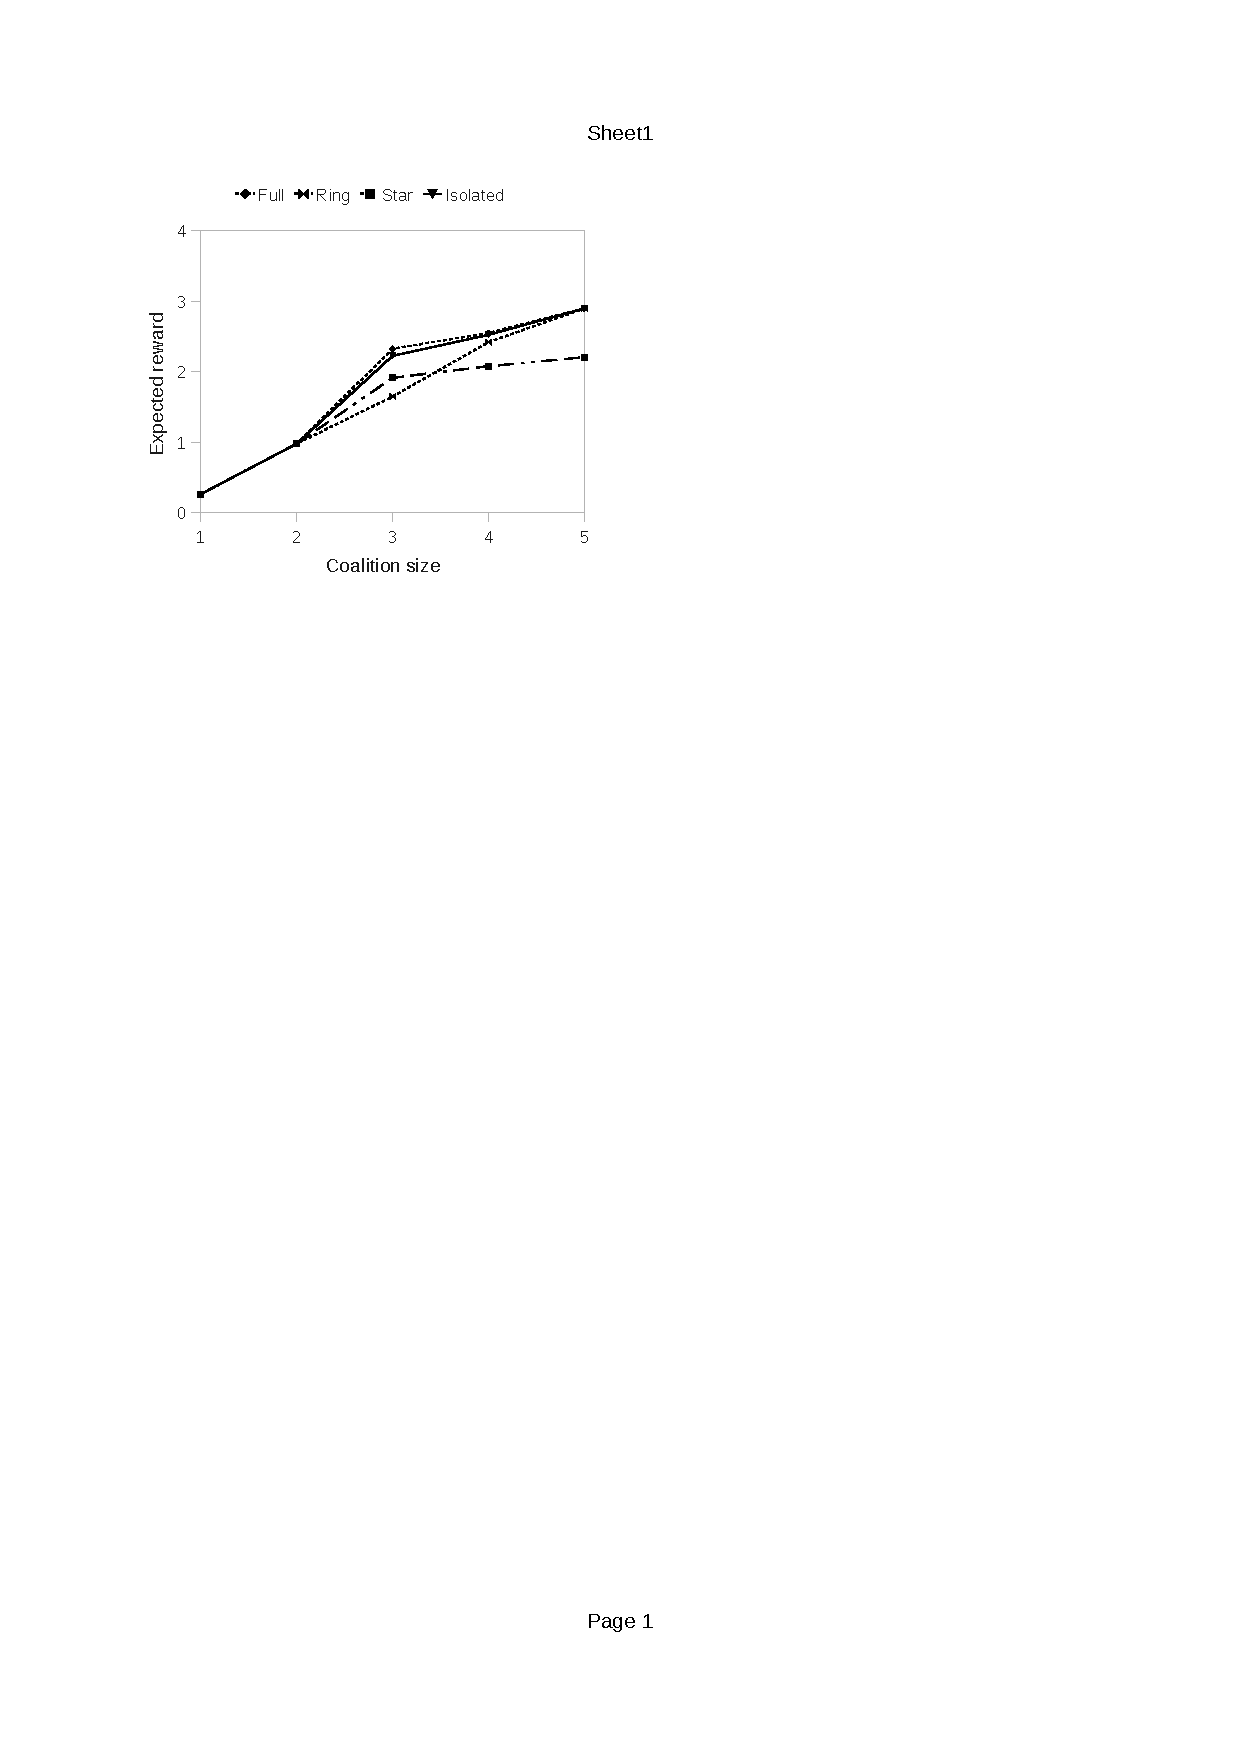
\includegraphics[clip=true, trim=78 523 320 112, scale=0.65]{images/w1_stpg_offline}
}
\subfloat[Online. Reward $W_1(O)$.]{\label{fig:on_w1}
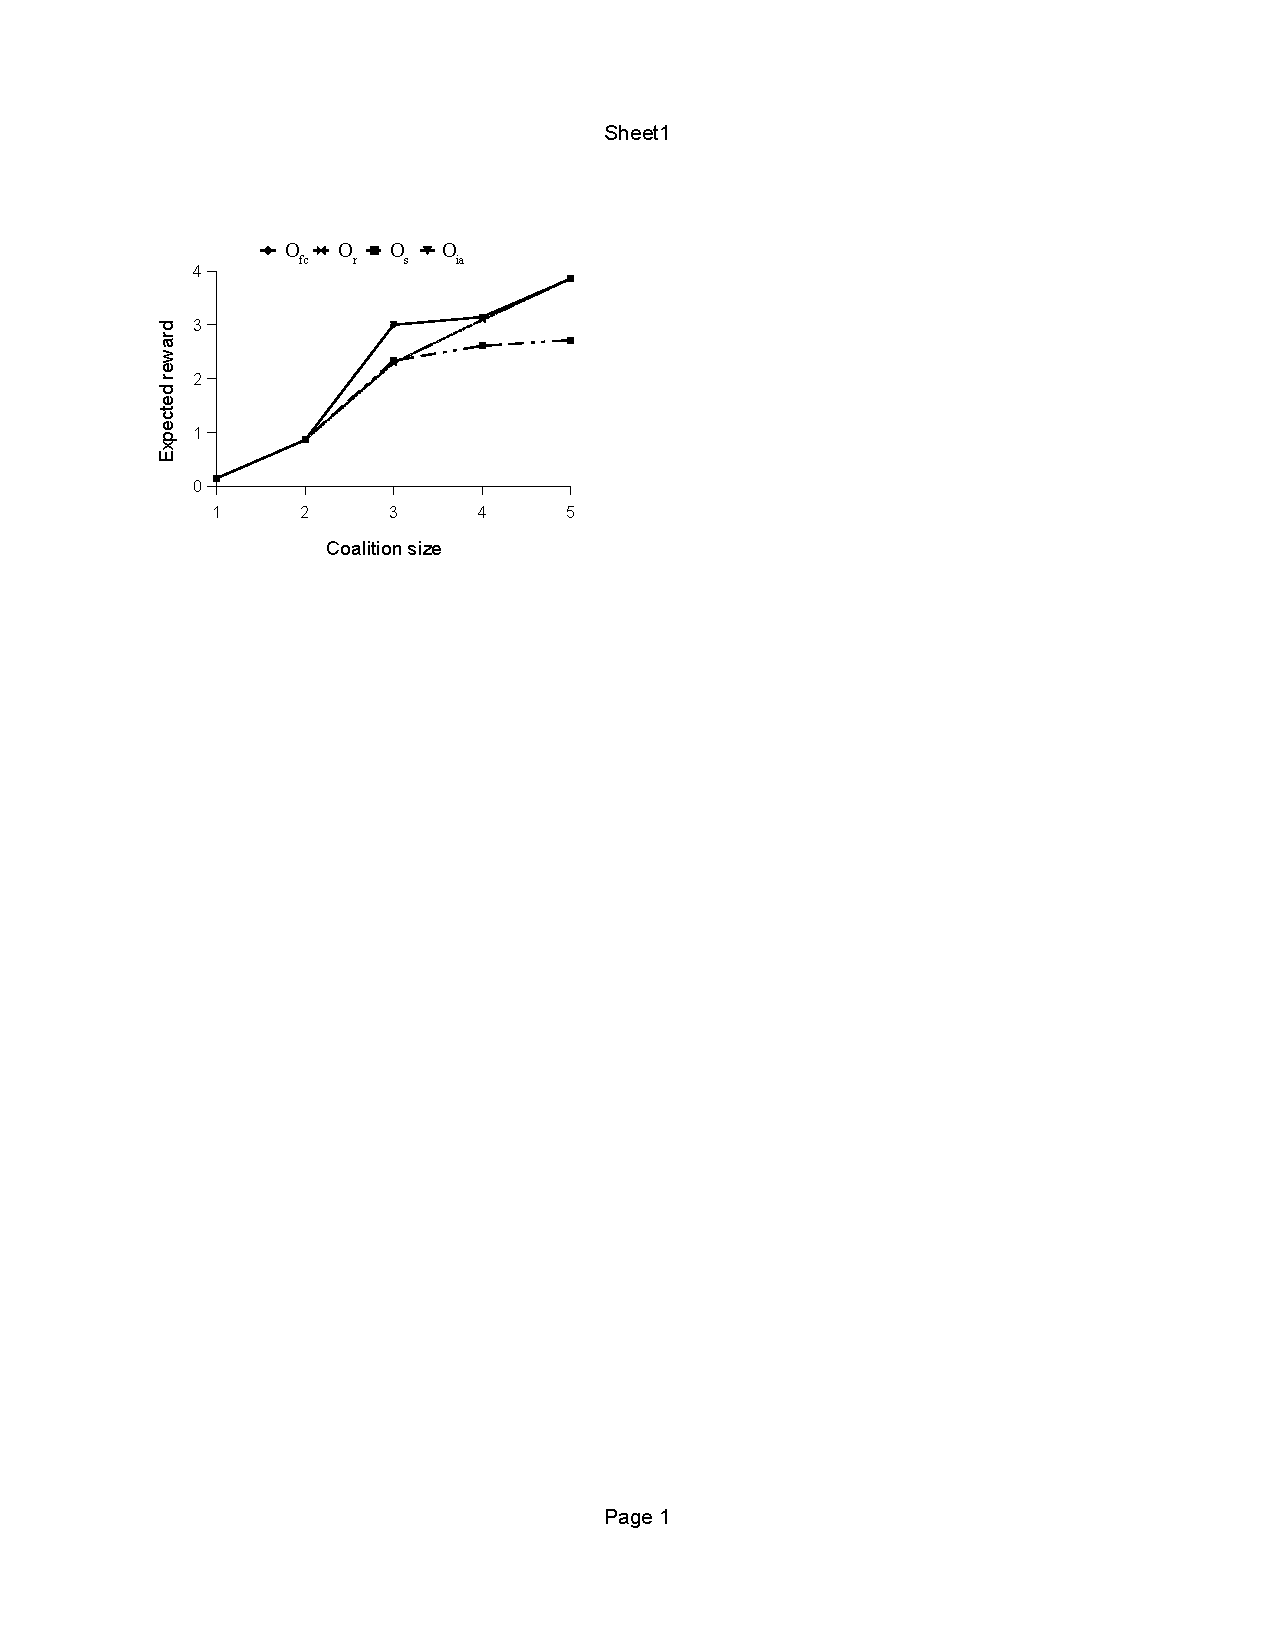
\includegraphics[clip=true, trim=70 520 280 112, scale=0.65]{images/w1_stpg_online}
}
\vspace{-8pt}

\ \ \ \ \ \ \ \ \ \ \ \subfloat[Offline. Reward $W_2(O)$.]{
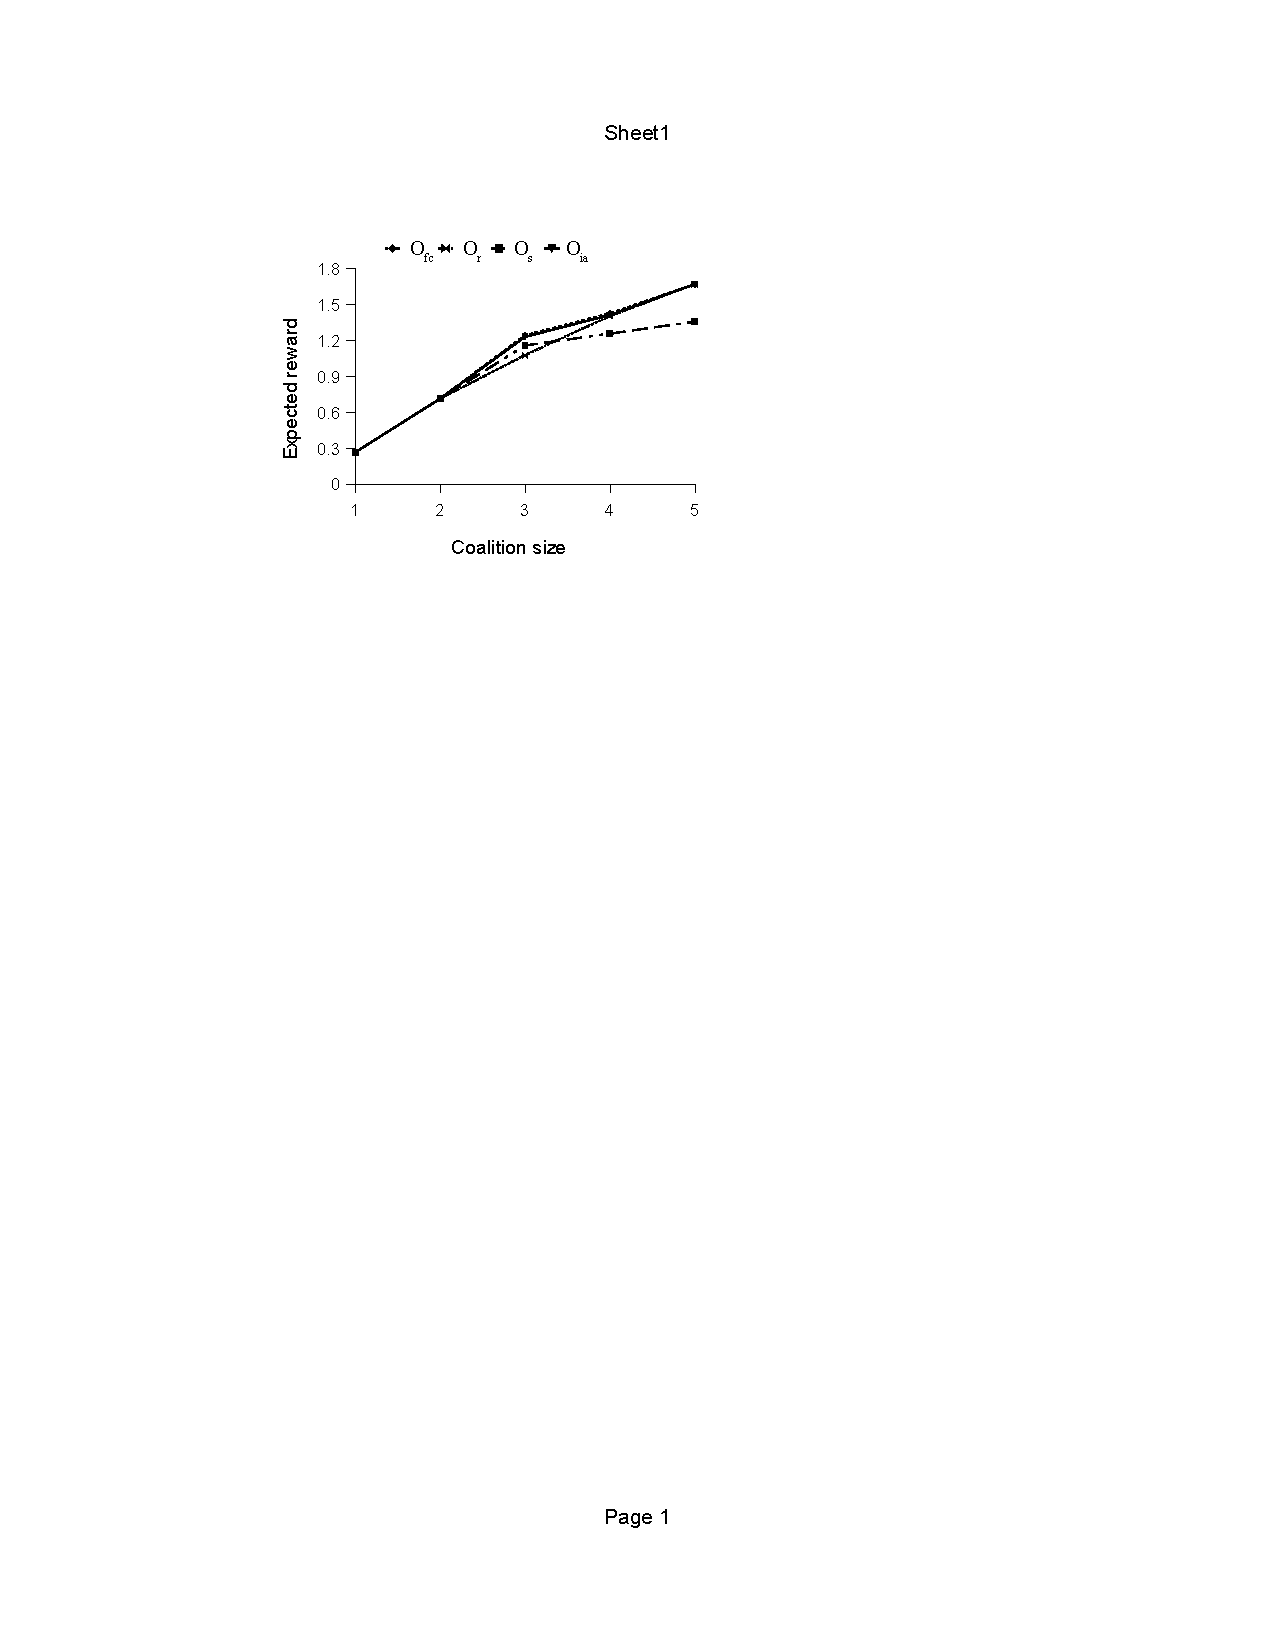
\includegraphics[clip=true, trim=137 520.5 270 115, scale=0.65]{images/w2_stpg_offline}
}
\subfloat[Online. Reward $W_2(O)$.]{
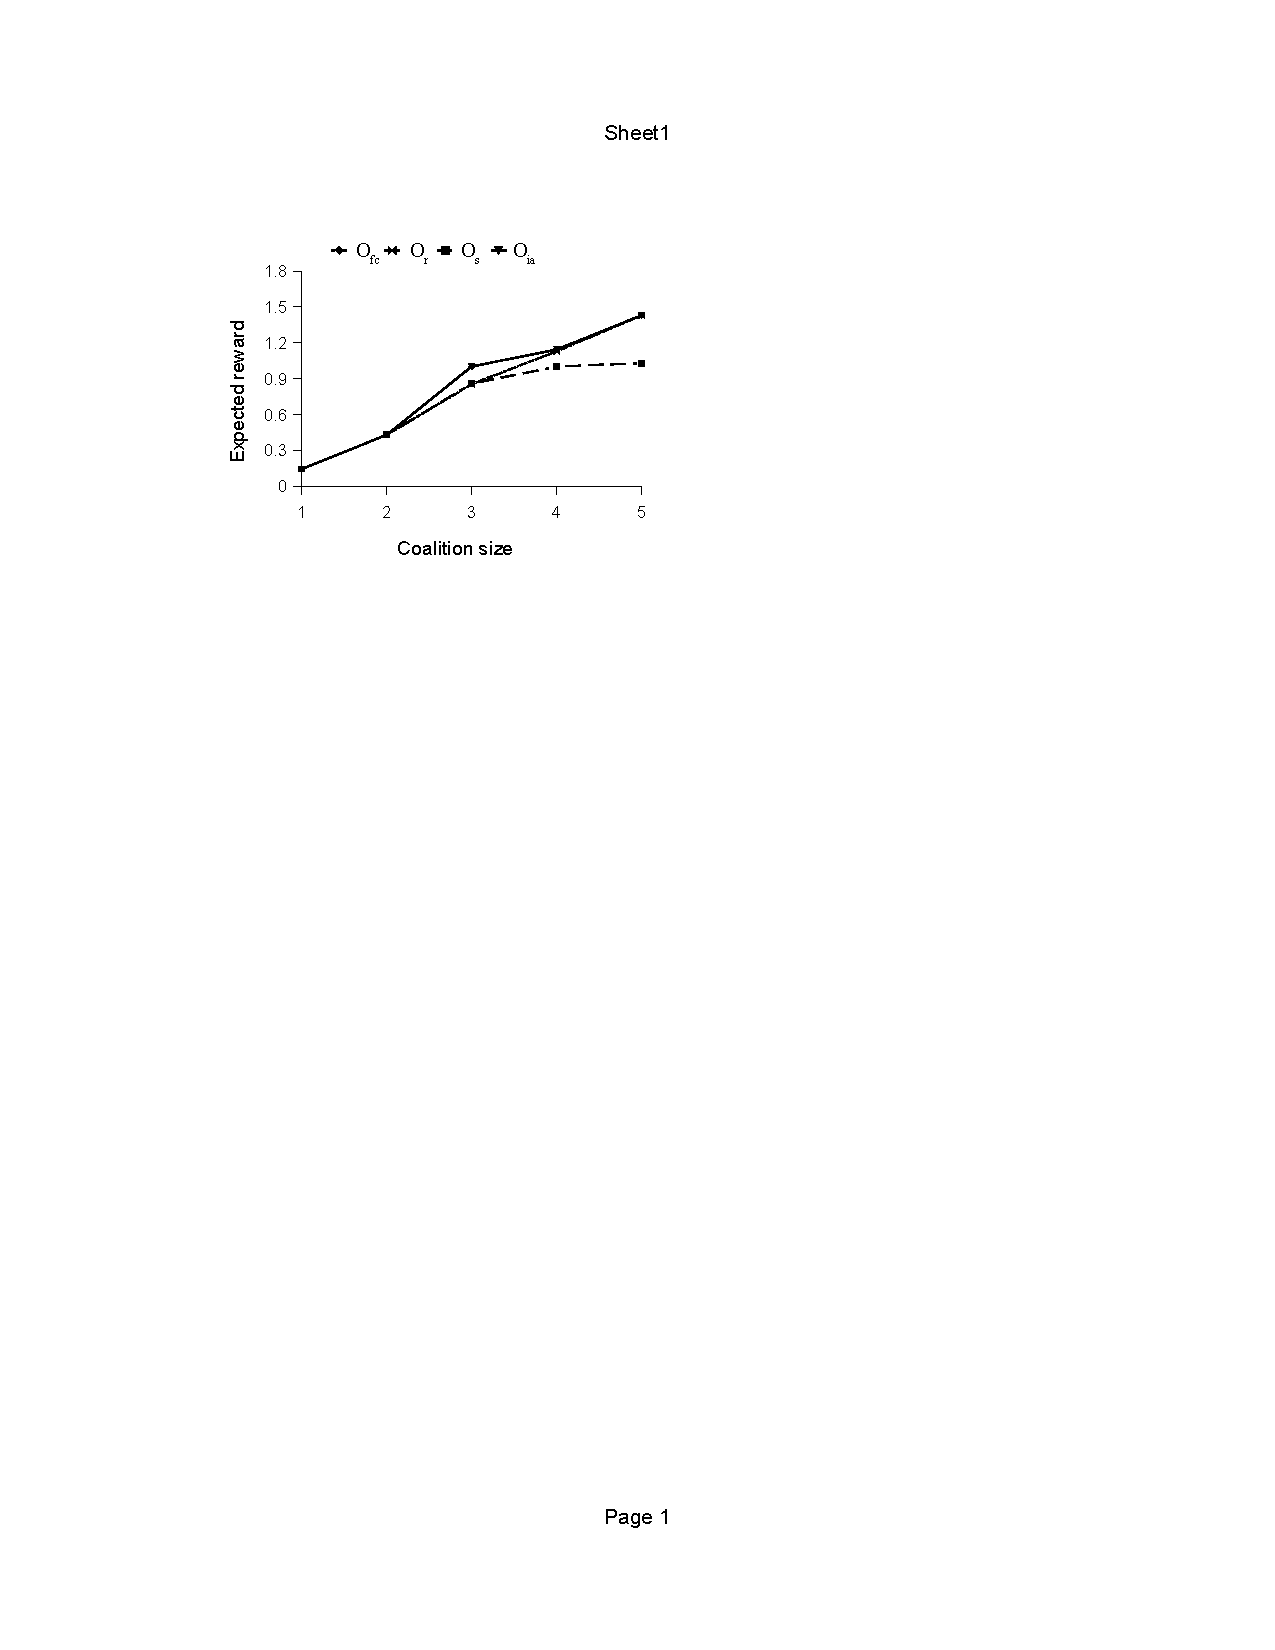
\includegraphics[clip=true, trim=101 520 280 115, scale=0.65]{images/w2_stpg_online}
}
\vspace{-8pt}
\caption{Graphs comparing how the optimal coalition's performance depends on its size. For precise data, see Tab. \ref{tab:opt_coa_reward_offline}-\ref{tab:opt_coa_reward_online} in Appendix \ref{app:coalitions_data}.}
\label{fig:coalition_performance}
\end{figure}


%Let us note that the strategy of an agent does not change when switching from offline to online setting, but it is the same strategy and the removal of constraint that the agent can only join a team for a task that it has the required skill for (which is obviously not known before the task is advertised) that results more agents joining teams. In the next section we will explore how the performance can be improved by changing the strategy of the agents so that they collaborate to optimise performance of the organisation.
%
For all agent organisations from Fig.~\ref{fig:network_configurations}, we enumerate all possible coalitions with different sizes use PRISM to compuite task completion probabilities (one task or both tasks) and rewards obtained ($W_1$ or $W_2$). These are done for both online and offline versions of the algorithm. It turns out that there exist coalitions of all sizes that are optimal with respect to all evaluated criteria; they are shown in Tab.~\ref{tab:optimal_coalitions}.
For detailed results please see Appendix \ref{app:coalitions_data}.



This result highlights the importance of positions in the network and resources held by the agents.
For example, agent $a_4$ is in all optimal coalitions of sizes greater than 1 for $O_{ia}$.
This is because it is connected to all agents, including agent $a_5$ which is isolated from other agents.
For $O_r$, however, the structure of the optimal coalition varies depending on coalition size. For example, for size 2 the optimal coalition consists of agents $a_2$ and $a_3$, but neither of them is in the optimal coalition of size 3.

\begin{table}
 \centering
 \begin{tabular}{ | l | l | l | l | l | l |}
    \hline
    $O$ & 1& 2 & 3 & 4 & 5 \\ \hline
    $O_{\mathit{fc}}$ & $\LD a_1 \RD$ & $\LD a_1, a_3 \RD$ & $\LD a_1, a_3, a_5 \RD$ & $\LD a_1, a_2, a_3, a_5 \RD$  & $\LD a_1, a_2, a_3, a_4, a_5 \RD$ \\ \hline
    $O_r$ & $\LD a_1 \RD$  & $\LD a_2, a_3 \RD$ & $\LD a_1, a_4, a_5 \RD$ & $\LD a_1, a_2, a_4, a_5 \RD$  & $\LD a_1, a_2, a_3, a_4, a_5 \RD$ \\ \hline
    $O_s$ & $\LD a_1 \RD$  & $\LD a_1, a_2 \RD$ & $\LD a_1, a_2, a_4 \RD$ & $\LD a_1, a_2, a_3, a_4 \RD$  & $\LD a_1, a_2, a_3, a_4, a_5 \RD$ \\ \hline
    $O_{ia}$ & $\LD a_1 \RD$  & $\LD a_1, a_4 \RD$ & $\LD a_1, a_2, a_4 \RD$ & $\LD a_1, a_2, a_4, a_5 \RD$  & $\LD a_1, a_2, a_3, a_4, a_5 \RD$ \\ \hline
\end{tabular}
\vspace{+2pt}
\caption{Optimal coalitions of all sizes for agent organisations from Fig.~\ref{fig:network_configurations}.}
\label{tab:optimal_coalitions}
\end{table}

Fig.~\ref{fig:coalition_performance} shows a comparison of agent organisations in terms of the maximum performance for different coalition sizes. $O_{\mathit{fc}}$ outperforms others in all examples. This is interesting, because it suggests that having strong connectivity within the team outweighs the exposure to many hostile agents. Performance of $O_r$ is the most consistent, as the maximum reward increases steadily with the coalition size.
However, to be as effective as more connected networks like $O_{\mathit{fc}}$, the coalition has to contain most agents in the network. Better performance of $O_s$ against $O_r$ for coalition sizes up to 3 illustrates the importance of having a highly interconnected agent for small coalitions.

Important differences between the online and offline settings can be seen for reward $W_1$ in Fig.~\ref{fig:off_w1} and \ref{fig:on_w1}. When going from coalition size 2 to 3, especially, for strongly connected $O_{\mathit{fc}}$ and $O_{ia}$, coalitions can ensure that one task is completed with probability 1.0 (see Tab.~\ref{tab:optimal_1task}), and thus guaranteeing reward of at least 3 for the coalition, which results in a jump of performance.


We have showed how an extension of PRISM to support STPGs can be used to verify properties of the multi-agent system that can be enforced by particular agent coalitions. This competitive  scenario allowed us to analyse the team formation algorithm from the coalitional perspective, finding the optimal coalitions and comparing their performance on different network topologies.

\vspace{-11pt}
\section{Conclusion and Future Work}
\vspace{-8pt}
In this paper, we have presented a comprehensive, formal analysis of a team formation algorithm using probabilistic model checking. We believe this demonstrates the strong potential of these techniques to the formal analysis of multi-agent systems and hope that this case study will serve as a motivation for further work in this area.

As ongoing and future work,
we plan to explore parallel execution of the \textsc{JoinTeam} algorithm for multiple agents, as here we only considered sequential execution, and consider the problem of synthesising optimal agent organisations for task distributions, from a mechanism design perspective.
We also plan to develop our prototype extension of PRISM
into a fully-fledged model checker for stochastic games
and to equip the analysis with abstraction techniques to allow for analysis of larger systems.

%\paragraph{Future work.} Although we have conducted a comprehensive analysis of the team formation protocol, many interesting directions and challenges remain as ongoing and future work. Here we simply outline some of them:
%\vspace{-5pt}
%\begin{itemize}

%\item Take advantage of abstraction techniques to extend the analysis to larger systems of agents.

%\item Verify ``dual" properties. For instance, rather than asking ``what is the expected reward'', we would like to be able to answer questions like ``what is the probability of reaching reward value $R$?''. This also applies to the strategy synthesis setting.

%\item Explore parallel execution of the \textsc{JoinTeam} algorithm for multiple agents, as here we only considered sequential execution. %(i.e. interleaving steps of JoinTeam algorithm
%    In particular, it would be interesting to investigate how this affects strategies of agents in both online and offline versions of the algorithm. %Also this raises many interesting scheduling problems, as worst and best case scheduling (of action interleaving) scenarios are unrealistic, the challenging question is to both develop realistic schedulers and perform model-checking efficiently.

 %\item Conducting experiments with agents having multiple resources, allowing agents to change teams until stable point is reached and check whether it can reached, what is the expected number of steps to reach the stable configuration, etc.

% \item Synthesise the optimal agent organisation given a set of tasks. % and their distributions.
 %      This problem turns out to be an instance of the mechanism design problem in game theory, where the designer can have control over neighbourhood structure or agent resources or both. We plan to attack this question by probabilistic model checking techniques.

%\end{itemize}
%\vspace{-20pt}


\small{

\begin{thebibliography}{10}

\bibitem{abdallah2004organization}
S. Abdallah and V.R. Lesser.
\newblock Organization-based cooperative coalition formation.
\newblock In {\em IAT}, pages 162--168. IEEE Computer Society, 2004.

\bibitem{agotnes2009reasoning}
T.~{\AA}gotnes, W.~van~der Hoek, and M.~Wooldridge.
\newblock {Reasoning about coalitional games}.
\newblock {\em Artificial Intelligence}, 173(1):45--79, 2009.

\bibitem{AlurHK02}
R. Alur, T.A. Henzinger, and O. Kupferman.
\newblock Alternating-time temporal logic.
\newblock {\em J. ACM}, 49(5):672--713, 2002.

\bibitem{BFW06b}
P.~Ballarini, M.~Fisher, and M.~Wooldridge.
\newblock Uncertain agent verification through probabilistic model-checking.
\newblock In {\em Proc. of SASEMAS'06}, 2006.

\bibitem{bonzon2007efficient}
E. Bonzon, M.-C. Lagasquie-Schiex, and J. Lang.
\newblock Efficient coalitions in {B}oolean games.
\newblock In {\em Texts in Logic
  and Games}, vol.5,
  pp. 293--297. 2008.

\bibitem{chatterjee2007strategy}
K.~Chatterjee, T.~Henzinger, and N.~Piterman.
\newblock {Strategy logic}.
\newblock In {\em Proc. CONCUR 2007}, LNCS 4703, pp. 59--73, Springer, 2007.

\bibitem{Con92}
A. Condon.
\newblock The complexity of stochastic games.
\newblock {\em Inf. Comput.}, 96(2):203--224, 1992.

\bibitem{dunne2008cooperative}
P.E. Dunne, W.~van~der Hoek, S.~Kraus, and M.~Wooldridge.
\newblock {Cooperative boolean games}.
\newblock In {\em Proc. of AAMAS'08}, pp. 1015--1022. ACM, 2008.

\bibitem{FKNP11}
V.~Forejt, M.~Kwiatkowska, G.~Norman, and D.~Parker.
\newblock Automated Verification Techniques for Probabilistic Systems.
\newblock In {\em Proc. SFM'11}, Springer, 2011. To appear.
%booktitle={Formal Methods for Eternal Networked Software Systems (SFM'11)},

\bibitem{gaston2005agent}
M.E. Gaston and M.~desJardins.
\newblock {Agent-organized networks for dynamic team formation}.
\newblock In {\em Proc. of AAMAS'05}, pp. 230--237. ACM, 2005.

\bibitem{glinton2008agent}
R.~Glinton, P.~Scerri, and K.~Sycara.
\newblock {Agent-based sensor coalition formation}.
\newblock In {\em Information Fusion, 2008 11th International Conference on},
  pp. 1--7. IEEE, 2008.

\bibitem{HJ94}
H.~Hansson and B.~Jonsson.
\newblock A logic for reasoning about time and reliability.
\newblock {\em Formal Aspects of Computing}, 6(5):512--535, 1994.

\bibitem{kraus2003coalition}
S.~Kraus, O.~Shehory, and G.~Taase.
\newblock {Coalition formation with uncertain heterogeneous information}.
\newblock In {\em Proc. of AAMAS'03}, pp. 1--8. ACM, 2003.

\bibitem{KN02}
M.~Kwiatkowska and G.~Norman.
\newblock Verifying randomized {Byzantine} agreement.
\newblock In {\em Proc. of FORTE'02}, {\em LNCS} 2529,
  pp. 194--209. Springer, 2002.

\bibitem{KNP07a}
M.~Kwiatkowska, G.~Norman, and D.~Parker.
\newblock Stochastic model checking.
\newblock In {\em Proc. SFM'07}, LNCS 4486, pp. 220--270. Springer, 2007.

\bibitem{KNP11}
M.~Kwiatkowska, G.~Norman, and D.~Parker.
\newblock PRISM 4.0: Verification of probabilistic real-time systems.
\newblock In {\em Proc. of CAV'11}, LNCS. Springer, 2011.
\newblock To appear.

\bibitem{lomuscio2006mcmas}
A.~Lomuscio and F.~Raimondi.
\newblock {MCMAS: A model checker for multi-agent systems}.
\newblock In {\em Proc. of TACAS'06}, LNCS 3920, pp. 450--454. Springer, 2006.

\bibitem{manisterski2006forming}
E.~Manisterski, E.~David, S.~Kraus, and N.R. Jennings.
\newblock {Forming efficient agent groups for completing complex tasks}.
\newblock In {\em Proc. of AAMAS'06}, pp. 834--841. ACM, 2006.

\bibitem{osborne1994course}
M.J. Osborne and A.~Rubinstein.
\newblock {\em {A course in game theory}}.
\newblock The MIT press, 1994.

\bibitem{shehory1998methods}
O.~Shehory and S.~Kraus.
\newblock {Methods for task allocation via agent coalition formation}.
\newblock {\em Artificial Intelligence}, 101(1-2):165--200, 1998.

\end{thebibliography}


}
%
%\bibliographystyle{plain}
%\bibliography{refs}



\clearpage
\appendix
\section{Formal Definitions of Agent Organizations}
\begin{itemize}
 \item Fully connected (Fig.~\ref{subfig:fully_connected}) $O_{\mathit{fc}}=\langle A, N_{fc}, R, R_{A_{fc}}  \rangle$ where
    \begin{itemize}
    \item $N_{fc}=\{\{a_i,a_j \}\ : 1 \le i,j \le 5, i\neq j \}$,
    \item $R_{A_{fc}}=\{R_{a_1}, R_{a_2}, R_{a_3}, R_{a_4}, R_{a_5}\}$ where $R_{a_1}=\{r_1\}$, $R_{a_2}=\{r_1\}$, $R_{a_3}=\{r_2\}$, $R_{a_4}=\{r_2\}$, and $R_{a_5}=\{r_3\}$.
    \end{itemize}
 \item Ring (Fig.~\ref{subfig:ring}) $O_r=\langle A, N_r, R, R_{A_r}  \rangle$ where
    \begin{itemize}
    \item $N_r=\{\{a_i,a_j \}\ : 1 \le i,j \le 5, i\neq j, i\le 5 \implies j=i+1, i=5 \implies j=1 \}$,
    \item $R_{A_r}=\{R_{a_1}, R_{a_2}, R_{a_3}, R_{a_4}, R_{a_5}\}$ where $R_{a_1}=\{r_1\}$, $R_{a_2}=\{r_2\}$, $R_{a_3}=\{r_1\}$, $R_{a_4}=\{r_2\}$, and $R_{a_5}=\{r_3\}$.
    \end{itemize}
 \item Star (Fig.~\ref{subfig:star}) $O_s=\langle A, N_s, R, R_{A_s}  \rangle$ where
    \begin{itemize}
    \item $N_s=\{\{a_i,a_j \}\ : 1 \le i,j \le 5, i\neq j, i=1 \}$,
    \item $R_{A_s}=\{R_{a_1}, R_{a_2}, R_{a_3}, R_{a_4}, R_{a_5}\}$ where $R_{a_1}=\{r_1\}$, $R_{a_2}=\{r_2\}$, $R_{a_3}=\{r_2\}$, $R_{a_4}=\{r_3\}$, and $R_{a_5}=\{r_3\}$.
    \end{itemize}
 \item Isolated agent (Fig.~\ref{subfig:isolated}) $O_{ia}=\langle A, N_{ia}, R, R_{A_{ia}}  \rangle$ where
    \begin{itemize}
    \item $N_{ia}=\{\{a_i,a_j \}\ : 1 \le i,j \le 5, i\neq j, (i=5 \vee j=5) \implies (i=4 \vee j=4) \}$,
    \item $R_{A_{ia}}=\{R_{a_1}, R_{a_2}, R_{a_3}, R_{a_4}, R_{a_5}\}$ where $R_{a_1}=\{r_1\}$, $R_{a_2}=\{r_2\}$, $R_{a_3}=\{r_3\}$, $R_{a_4}=\{r_3\}$, and $R_{a_5}=\{r_2\}$.
    \end{itemize}
\end{itemize}
\clearpage

\iffalse
\section{PRISM Language}
\label{sec:prism_lang}
The basic components of the language are modules and variables. A
system is constructed as a number of modules which can interact with each other.
A module contains a number of variables which express the state of the module,
and its behaviour is given by a set of guarded commands of the form:

[] $\langle$guard$>$ \! $\langle$command$>$;

The guard is a predicate over the variables of the system and the command describes
a transition which the module can make if the guard is true (using primed variables
to denote the next values of variables). If a transition is probabilistic, then the
command is specified as:

$\langle prob \rangle$ : $\langle$ command $\rangle$ + ...+ $\langle$ prob$\rangle$ : <command>
\fi

\section{State Transition System} \label{app:transitions}
\begin{figure}
  \centering
  \vspace{-50pt}
	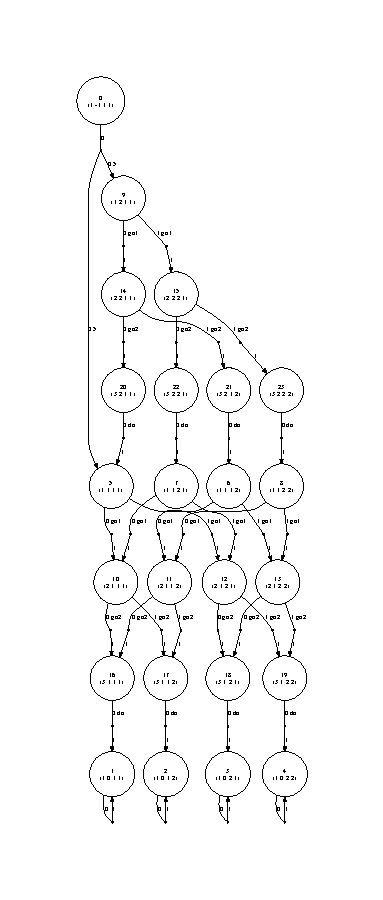
\includegraphics[]{images/transition_system}
	\vspace{-35pt}
	\caption{State transition system of the model from Figure \ref{fig:prism_example} generated by PRISM.}
\end{figure}
\clearpage
\section{Data for STPG Analysis}
\label{app:coalitions_data}

Tab.~\ref{tab:optimal_1task} shows the maximum probability for completion of one task, whereas Tab.~\ref{tab:optimal_2task} shows the maximum probability for completion of two tasks; both contain the online and offline versions. It is also interesting to see that for the coalition consisting of one agent, it has a positive probability to accomplish one task, but cannot accomplish two tasks for all four organizations.




\begin{table}
 \centering
\subfloat[Offline]{
  \begin{tabular}{ | l | l | l | l | l | l |}
      \hline
      $O$ & 1 & 2 & 3 & 4 & 5 \\ \hline
      $O_{\mathit{fc}}$ & 0.14285 & 0.42857 & 1.0 & 1.0 & 1.0  \\ \hline
      $O_r$ & 0.14285 & 0.42857 & 0.68333 &  0.92619 & 1.0 \\ \hline
      $O_s$ & 0.14285 & 0.42857 & 0.79761 & 0.81904 & 0.82857\\ \hline
      $O_{ia}$ & 0.14285 & 0.42857 & 0.93452 & 1.0 & 1.0\\ \hline
  \end{tabular}
}
\subfloat[Online]{
  \begin{tabular}{ | l | l | l | l | l | l |}
      \hline
      $O$ & 1 & 2 & 3 & 4 & 5 \\ \hline
      $O_{\mathit{fc}}$ & 0.14285 & 0.42857 & 1.0 & 1.0 & 1.0  \\ \hline
      $O_r$ & 0.14285 & 0.33333 & 0.68571 & 0.89523 & 1.0 \\ \hline
      $O_s$ & 0.14285 & 0.42857 & 0.76190 & 0.84761 & 0.88571 \\ \hline
      $O_{ia}$ & 0.14285 & 0.42857 & 0.92857 & 1.0 & 1.0\\ \hline
  \end{tabular}
}
\caption{Values for maximum probabilities to complete one task for coalitions from Tab.~\ref{tab:optimal_coalitions}.} \label{tab:optimal_1task}
\end{table}


\begin{table}
 \centering
\subfloat[Offline]{
 \begin{tabular}{ | l | l | l | l | l | l |}
    \hline
    $O$ & 1 & 2 & 3 & 4 & 5 \\ \hline
    $O_{\mathit{fc}}$ & 0.0 & 0.04081 & 0.24489 &  0.42857 & 0.67346  \\ \hline
    $O_r$ & 0.0 &  0.04081 & 0.17687 & 0.40748 & 0.67346\\ \hline
    $O_s$ & 0.0 & 0.04081 & 0.20408 & 0.29523 & 0.39183 \\ \hline
    $O_{ia}$ & 0.0 & 0.04081 & 0.23129 & 0.41496 & 0.67346\\ \hline
\end{tabular}
}
\subfloat[Online]{
 \begin{tabular}{ | l | l | l | l | l | l |}
    \hline
    $O$ & 1 & 2 & 3 & 4 & 5 \\ \hline
    $O_{\mathit{fc}}$ & 0.0 & 0.02040 & 0.06122 &  0.18367 & 0.42857  \\ \hline
    $O_r$ & 0.0 & 0.02040 & 0.06122 & 0.18367 & 0.42857\\ \hline
    $O_s$ & 0.0 & 0.02040 & 0.06122 & 0.12244 & 0.12653 \\ \hline
    $O_{ia}$ & 0.0 & 0.02040 & 0.06122 & 0.18231 & 0.42857\\ \hline
\end{tabular}
}

\caption{Values for maximum probabilities to complete both tasks for coalitions from Tab.~\ref{tab:optimal_coalitions}.} \label{tab:optimal_2task}
\end{table}



Tab.~\ref{tab:opt_coa_reward_offline} and Tab.~\ref{tab:opt_coa_reward_online} show the maximum ($W_1$/$W_2$) rewards in the offline and online versions respectively.


\begin{table}
 \centering
 \begin{tabular}{ | l | l | l | l | l | l |}
    \hline
    $O$ & 1& 2 & 3 & 4 & 5 \\ \hline
    $O_{\mathit{fc}}$ & 0.26530/0.26530  & 0.97959/0.71428  &  2.32653/1.24489  &  2.55102/1.42857   &  2.89795/1.67346  \\ \hline
    $O_r$ &  0.26530/0.26530   & 0.97959/0.71428  &  1.64897/1.07891  &  2.41972/1.40680   &  2.89795/1.67346 \\ \hline
    $O_s$ &  0.26530/0.26530   &  0.97959/0.71428  & 1.91496/1.15986  &  2.07857/1.25884   &  2.20816/1.35918  \\ \hline
    $O_{ia}$ & 0.26530/0.26530   &  0.97959/0.71428  &  2.22619/1.23129  &  2.52380/1.41496   &  2.89795/1.67346  \\ \hline
\end{tabular}
\caption{Performance of optimal coalitions from Tab.~\ref{tab:optimal_coalitions} for offline version using rewards $W_1$/$W_2$.}
\label{tab:opt_coa_reward_offline}
\end{table}


\begin{table}
 \centering
 \begin{tabular}{ | l | l | l | l | l | l |}
    \hline
    $O$ & 1& 2 & 3 & 4 & 5 \\ \hline
    $O_{\mathit{fc}}$ &   0.14285/0.14285  &  0.85714/0.42857  &  2.99999/0.99999  &  3.14285/1.14285   &  3.85714/1.42857  \\ \hline
    $O_r$ &  0.14285/0.14285   &  0.85714/0.42857  &  2.29047/0.85238  &  3.08928/1.12738   &  3.85714/1.42857  \\ \hline
    $O_s$ &  0.14285/0.14285   &  0.85714/0.42857  &  2.33333/0.85714  &   2.60714/0.99999   &  2.71428/1.02857  \\ \hline
    $O_{ia}$ &  0.14285/0.14285   &  0.85714/0.42857  &  2.99999/0.99999  &  3.14285/1.14285   &  3.85714/1.42857  \\ \hline
\end{tabular}
\caption{Performance of optimal coalitions from Tab.~\ref{tab:optimal_coalitions} for online version using rewards $W_1$/$W_2$.}
\label{tab:opt_coa_reward_online}
\end{table}

%\begin{table}
% \centering
% \begin{tabular}{ | l | l | l | l | l | l |}
%    \hline
%    $O$ & 1& 2 & 3 & 4 & 5 \\ \hline
%    $O_{\mathit{fc}}$ & 0.26530/0.26530  & 0.97959/0.71428  &  2.32653/1.24489  &  2.55102/1.42857   &  2.89795/1.67346  \\ \hline
%    $O_r$ &  0.26530/0.26530   & 0.97959/0.71428  &  1.64897/1.07891  &  2.41972/1.40680   &  2.89795/1.67346 \\ \hline
%    $O_s$ &  0.26530/0.26530   &  0.97959/0.71428  & 1.91496/1.15986  &  2.07857/1.25884   &  2.20816/1.35918  \\ \hline
%    $O_{ia}$ & 0.26530/0.26530   &  0.97959/0.71428  &  2.22619/1.23129  &  2.52380/1.41496   &  2.89795/1.67346  \\ \hline
%\end{tabular}
%\caption{Optimal coalitions of all for agent organisations from Fig.~\ref{fig:network_configurations} for offline version using rewards $W_1$/$W_2$.}
%\label{tab:optimal_coalitions}
%\end{table}



\end{document}
